% Author: Matthew Turner

\documentclass[11pt,letterpaper]{article}
% \documentclass[11pt]{report}
% \documentclass{report}
% \documentclass{book}
\usepackage[bookmarks]{hyperref}
\usepackage{amssymb,amsmath}
% \usepackage{fullpage}
\usepackage{tabulary}
\usepackage{tabularx}

% \usepackage[margin=1.00in]{geometry}
\usepackage[margin=0.90in]{geometry}
\usepackage{float}

\usepackage{caption}
\usepackage{booktabs}
\usepackage{pslatex}
\usepackage{apacite}
\usepackage{subcaption}
\usepackage{pgfplots}
\usepackage{wrapfig}
\usepackage[english]{babel}
\usepackage{lmodern}
\usepackage{setspace}
\doublespace
% \usepackage{url}
\usepackage{bigfoot}
\usepackage[export]{adjustbox}
\setlength\intextsep{0pt}
\hypersetup{linktocpage}

\usepackage{graphicx}

\title{\vspace{-1in}Identity signaling model progress}

\author{} %{Matthew A.~Turner}}

\begin{document}
\maketitle
\tableofcontents

\section{Introduction}

(JUST SOME SKETCHY/INCOMPLETE/INCORRECT NOTES MOSTLY FOR MYSELF)

Relationship between sending and receiving strategies in signaling: 
sending strategies in this model are \emph{overt} and \emph{covert}; 
receiving strategies are \emph{generous} and \emph{churlish}. We assume
that agents first signal their traits according to their sending strategy,
and receive signals from other individuals according to their receiving
strategy. These signals, in combination with the strength of homophily in
partner selection, determine the payoff received by two agents when they
interact. After one round of signaling and 10 rounds of interaction, agents
homophilically select another agent as their teacher, and adopt either their 
teacher's sending or receiving strategy with probability proportional to how
much greater the teacher's accumulated payoffs are than the learner's. 

While strategies evolve in this model, traits do not. All agents have 
$K$ binary traits of value $\pm1$ assigned at random at model initialization.
While $K$ could be set to any value, so far we have only studied $K=3$.
In the basic results and invasion experiment results below, all agent traits
are assigned by a coin flip. In the minority experiment, one of $K=3$ traits
are set to $+1$ for some minority fraction of agents, and the majority 
get a trait value of $-1$ for that trait. Trait values determine whether or
not agents are \emph{similar} or \emph{dissimilar}, which results in 
different payoffs (see Appendix Table ??). 

If agents signal overtly, they show other agents their traits openly, whether or
not they are similar or dissimilar. Covert signalers, on the other hand, 
are able to conceal their dissimilarity from their interaction partners, 
giving no information away if they are dissimilar, and showing similar traits
if their interaction partner is indeed similar. 

The degree of similarity of two agents determines the probability that two 
agents will interact, modulated by homophily, $w$.

The above process accounts for one model timestep/iteration. We found by
inspection that equilibrium occurs by 500 timesteps, so all heatmaps aggregate
over the 500th timestep (see Figure ?? in the Appendix). 

\section{Results}

\subsection{Basic results starting from equilibrium}

\subsection{Invasion}

In this experiment we begin with initial proportions, $\rho$ of one of the strategies
at 0.05 and consider this the ``invading'' strategy. $\rho_{cov,0}$ represents
the initial covert proportion, $\rho_{ov,0}$ the initial overt proportion,
$\rho_{ch,0}$ the initial churlish proportion, and $\rho_{gen,0}$ the 
initial generous proportion. We measure how often
a non-zero proportion of agents with the invading strategy manage to 
establish a permanent population, which we call invasion success. We calculated
invasion success for a number of experimental parameter settings, covarying
over disliking penalty ($d=\delta$) and homophily ($w$) in the first case,
and over relative covert receptivity ($r/R$) and homophily ($w$) 
in the second case (Figures~\ref{fig:cov-ov-invade} and~\ref{fig:ch-gen-invade}).

\begin{figure}[H]
  \centering
    \begin{subfigure}{0.49\textwidth}
      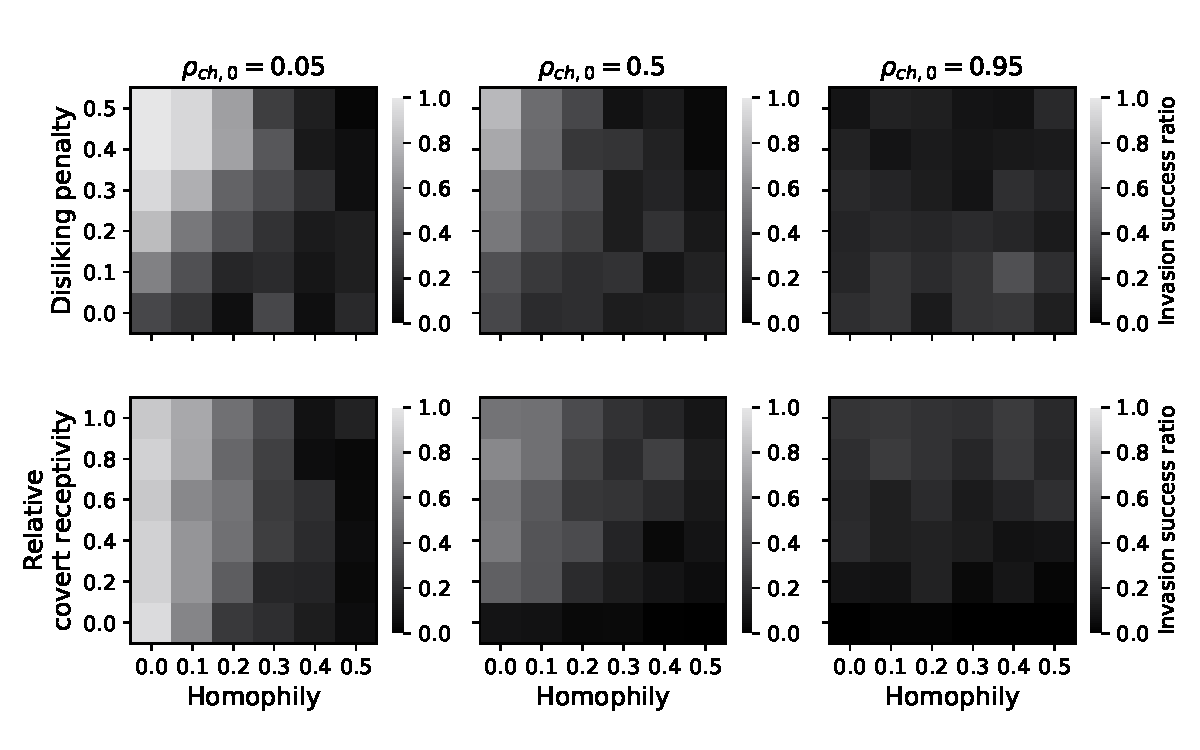
\includegraphics[width=\textwidth]{Figures/covert_invades.pdf}
      \caption{Covert invades, $\rho_{cov,0}=0.05$}
    \end{subfigure}
    \begin{subfigure}{0.49\textwidth}
      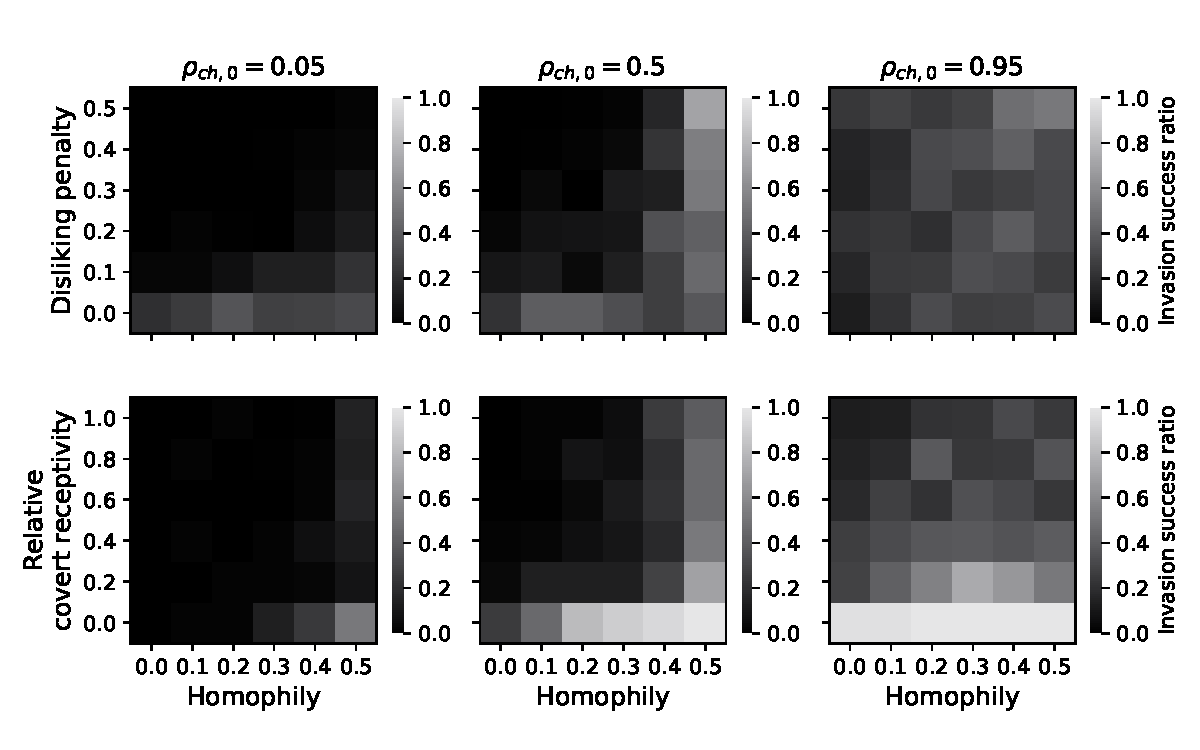
\includegraphics[width=\textwidth]{Figures/overt_invades.pdf}
      \caption{Overt invades, $\rho_{cov,0}=0.95$}
    \end{subfigure}
  \caption{Covert and overt sending strategy invasion success rates. 
    Lower homophily is more favorable for successful covert signaling invasion.
    This is due to lower homophily meaning agents cannot assort well into
    similar pairs prior to interaction.
    Similarly, greater homophily is more favorable for successful overt
    signaling invasion, where agents can better assort if they know each other's
    true traits. Unexpectedly, as covert receptivity increases, overt signaling
    is is more successful at invading and covert signaling is less successful
    at invading when the initial churlishness is high. When initial
    churlishness is small to moderate, the pattern is reversed.
  }
  \label{fig:cov-ov-invade}
\end{figure}

\begin{figure}[H]
  \centering
    \begin{subfigure}{0.49\textwidth}
      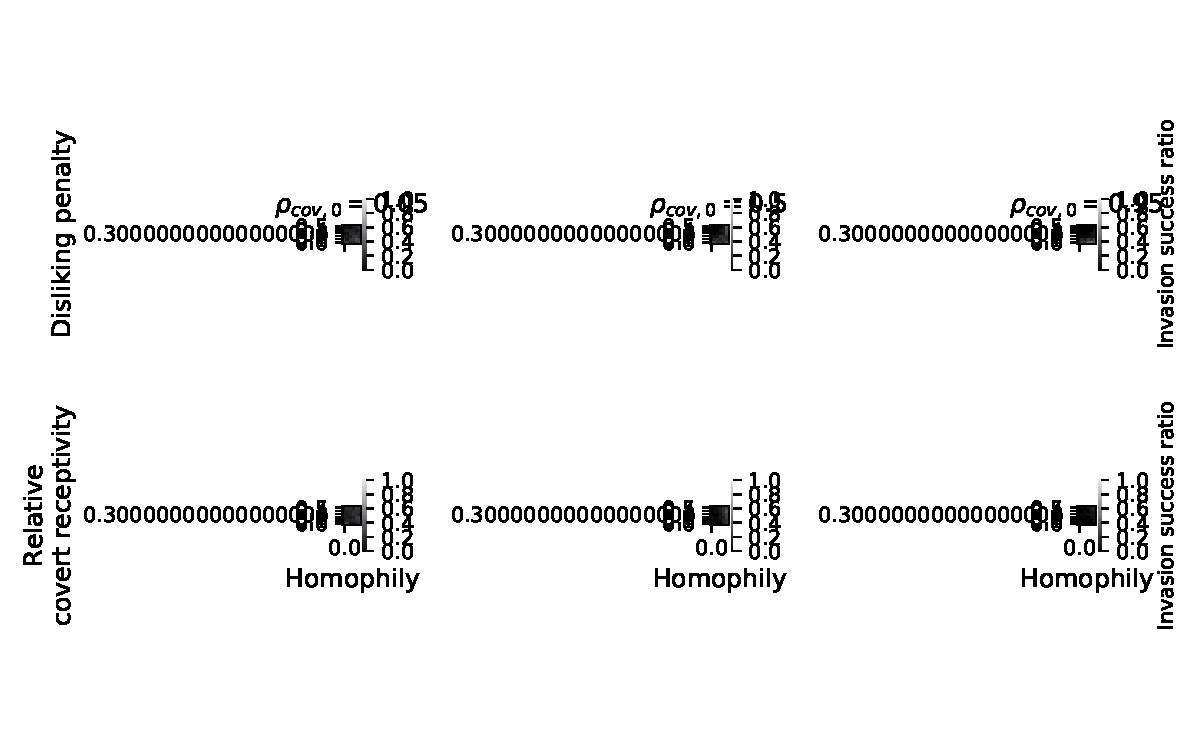
\includegraphics[width=\textwidth]{Figures/churlish_invades.pdf}
      \caption{Churlish invades, $\rho_{ch,0}=0.05$}
    \end{subfigure}
    \begin{subfigure}{0.49\textwidth}
      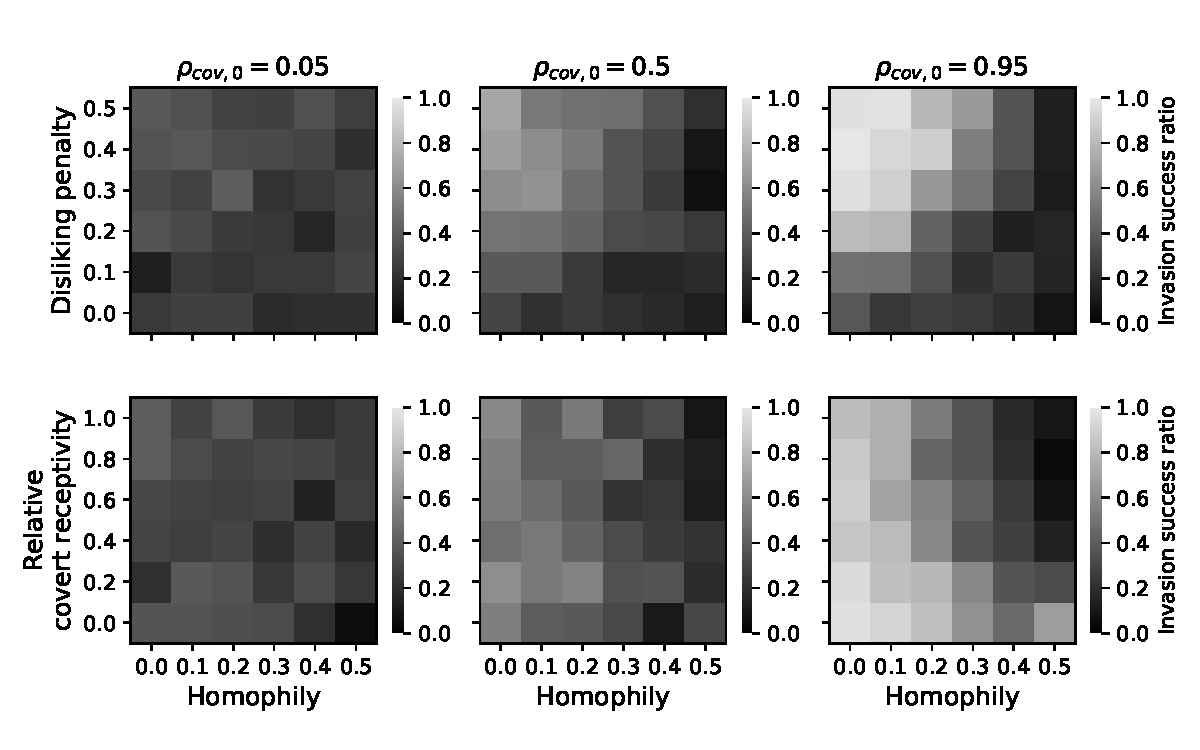
\includegraphics[width=\textwidth]{Figures/generous_invades.pdf}
      \caption{Generous invades, $\rho_{ch,0}=0.95$}
    \end{subfigure}
  \caption{Churlish and generous receiving strategy invasion success rates.
    For low to moderate rates of initial covert signaling there is not much
    of a pattern to invasion success. High values of homophily do seem to lead
    to more successful churlish invasion for moderate values of initial
    covert signalers. For large initial proportions of covert
    signalers, lower homophily favors generous invasion, which is more pronounced
    for larger disliking penalties.
  }
  \label{fig:ch-gen-invade}
\end{figure}




\subsection{Minority populations}


\appendix

\section{Evolution in signaling and receiving strategies}

For these preliminary results I focus on the evolution of signaling strategies,
each agent at model initialization. There are two output measures in these experiments:
density of covert signalers and density of churlish receivers. 
There are confirmatory results for two computational experiments in which I: 
(1) varied relative covert receptivity $r/R$ and 
homophily, $w$; and (2) varied the disliking penalties set equal, $d=\delta$,
and homophily, $w$.

The bonus payoff for two 
interacting agents where at least one
likes the other is set fixed to $s=0.25$. The payoff structure is as follows

\begin{table}[H]
  \centering
  \begin{tabular}{rcc}
    Attitude combo. & Payoff (similar) & Payoff (dissim.) \\
   \toprule
    Like/like & $1 + s$                    & NA \\
    Like/neutral & $1 + s$                 & NA \\
    Like/dislike & $1 + s - d$             & NA \\
    Neutral/neutral & 1 + s                & 1  \\
    Dislike/neutral & $1 + s - d$          & $1-d$\\
    Dislike/dislike & $1 + s - d - \delta$ & $1 - d - \delta$
  \end{tabular}
\end{table}

Agents only interact with one another with probability given by their attitudes
towards one another. If two agents are assorted together to potentially 
interact, these are the probabilities the agents do interact.

\begin{table}[H]
  \centering
  \begin{tabular}{rc}
    Attitudes & Pr(paired agents interact) \\
    \toprule
    Like/like & $0.5 + w$ \\
    Like/neutral & $0.5 + \frac{w}{2}$ \\
    Like/dislike & $0.5$ \\
    Neutral/neutral & $0.5$ \\
    Dislike/neutral & $0.5 - \frac{w}{2}$ \\
    Dislike/dislike & $0.5 - w$ 
  \end{tabular}
\end{table}

\subsection{Density of covert signalers vs. $r/R$ and homophily, $w$}

Based on results from ``Evolution of covert signaling'' (``ECS''), I designed
the first agent-based model experiment to determine the dependence of the
density of covert signalers in the population ($\rho_C$) on
the receptiveness of the population to covert signals ($r$) and the
importance of homophily ($w$) to assortment. 

Here I set $R=0.5$, $s=0.25$, $d=\delta=0.25$,
and $N=100$. After signaling, agents go through 10 rounds of assortment/interaction,
followed by evolution after the 10 rounds of interaction. The model has been
run out to 100 timesteps where timeseries are nearly stable, though we will
want more timesteps for our final study, or perhaps adjust the number of 
assortment/interaction rounds up or down per timestep, to guarantee full 
stability.

I systematically varied $r/R$ by setting $R=0.5$ and varied 
$r \in \{0.0, 0.05, 0.1, \ldots, 0.45\}$ to get $r/R \in \{0.0, 0.1, \ldots, 0.9\}$.
I varied homophily identically to $r$, $w \in \{0.0, 0.5, \ldots, 0.45\}$. Note
that both $r$ and $w$ are bounded above by 0.5.

\begin{figure}[H]

  \centering
  \begin{subfigure}{0.49\textwidth}
    \centering
    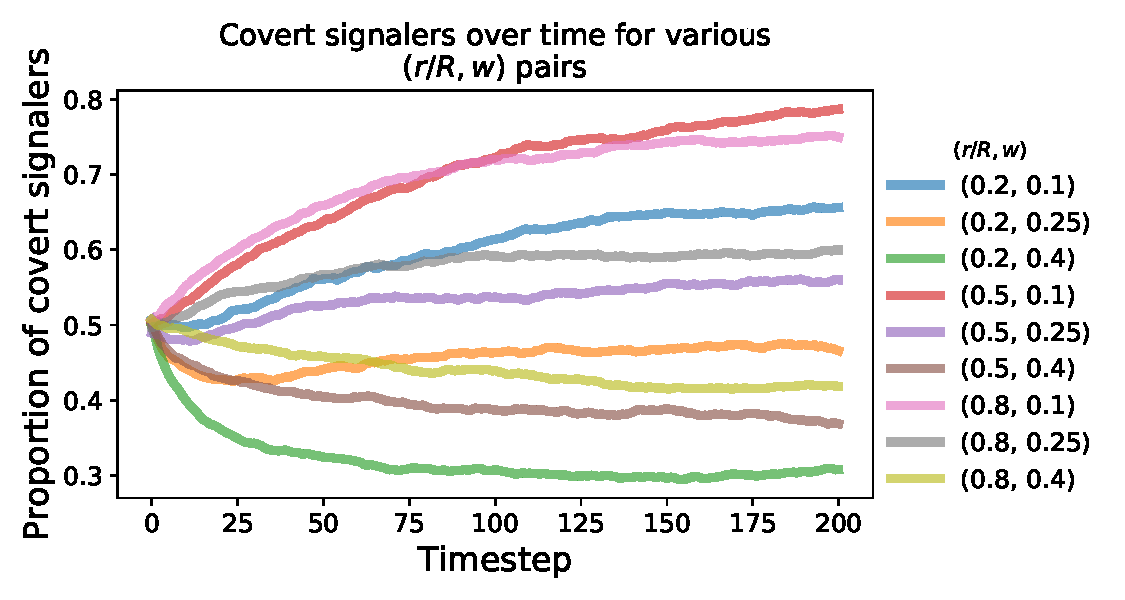
\includegraphics[width=\textwidth]{prelim/Figures/receptivityHomophilyCovertSeries.pdf}
    \caption{Density of covert signalers.}
  \end{subfigure}
  \begin{subfigure}{0.49\textwidth}
    \centering
    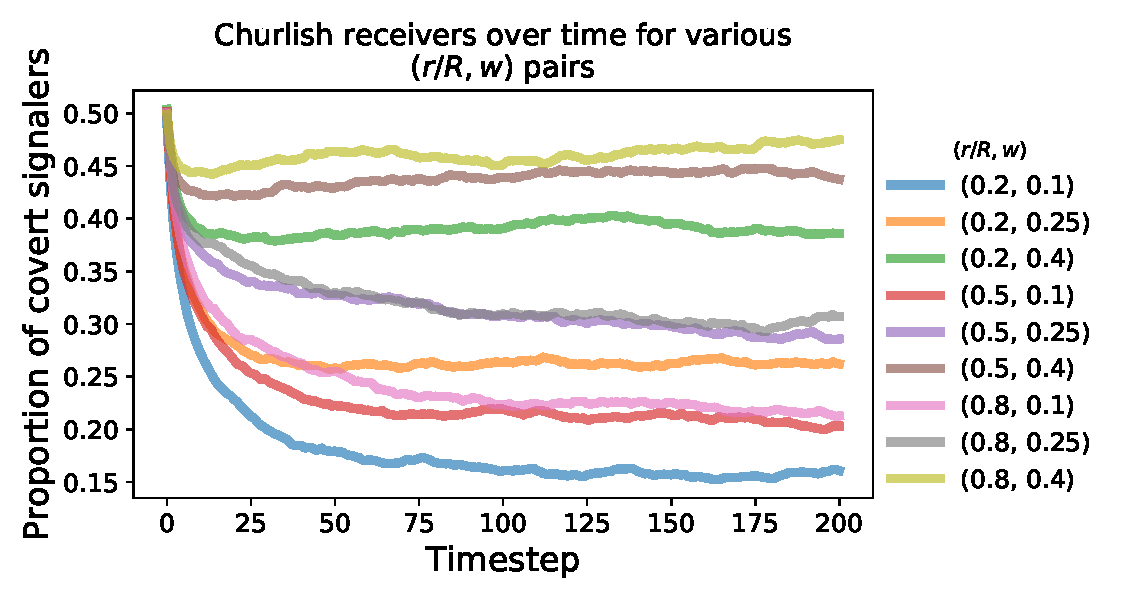
\includegraphics[width=\textwidth]{prelim/Figures/receptivityHomophilyChurlishSeries.pdf}
    \caption{Density of churlish receivers.}
  \end{subfigure}
  
  \caption{Timeseries of density of covert signalers and churlish receivers
    for nine combinations of $r$ and $w$. Receptivity of
    overt signals is $R=0.5$.}
  \label{fig:dislikingHomophilySeries}
\end{figure}

\begin{figure}[H]
  \centering
  \begin{subfigure}{0.49\textwidth}
    \centering
    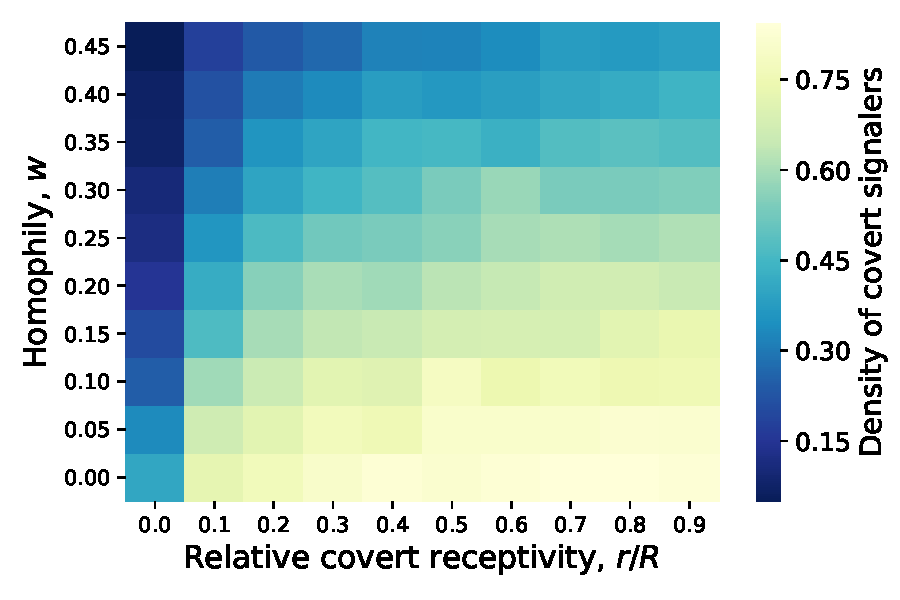
\includegraphics[width=\textwidth]{prelim/Figures/covertDensityVsReceptivityHomophilyCoevo.pdf}
    \caption{Density of covert signalers.}
  \end{subfigure}
  \begin{subfigure}{0.49\textwidth}
    \centering
    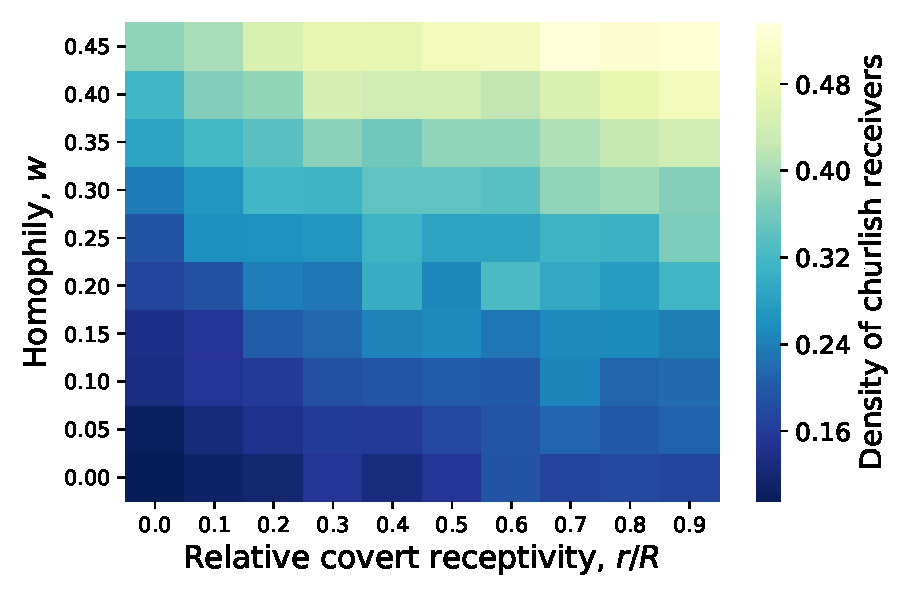
\includegraphics[width=\textwidth]{prelim/Figures/churlishDensityVsReceptivityHomophilyCoevo.pdf}
    \caption{Density of churlish receivers.}
  \end{subfigure}
  
  \caption{Density of covert signalers and churlish receivers at $t=200$, 
    final timestep recorded in this preliminary experiment. Receptivity of
    overt signals is $R=0.5$.}
  \label{fig:dislikingHomophilyHeatmap}
\end{figure}


\subsection{Density of covert signalers vs. disliking penalty $d=\delta$ and homophily, $w$}

Here I co-vary the disliking penalties, which I set equal ($d=\delta$), and
homophily, $w$. Here, $r=0.25$ and $R=0.5$. 

Specifically, I vary $d=\delta \in \{0.0, 0.05, 0.1, \ldots, 0.45\}$
As in the above experiment, I set $w \in \{0.0, 0.5, \ldots, 0.45\}$.

\begin{figure}[H]

  \centering
  \begin{subfigure}{0.49\textwidth}
    \centering
    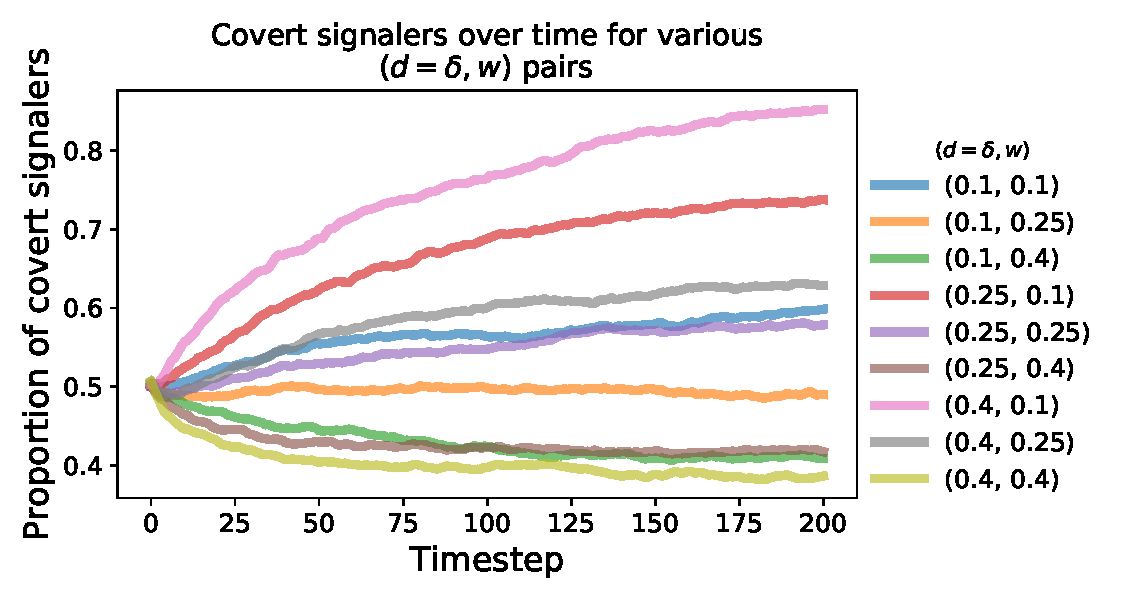
\includegraphics[width=\textwidth]{prelim/Figures/dislikingHomophilyCovertSeries.pdf}
    \caption{Density of covert signalers.}
  \end{subfigure}
  \begin{subfigure}{0.49\textwidth}
    \centering
    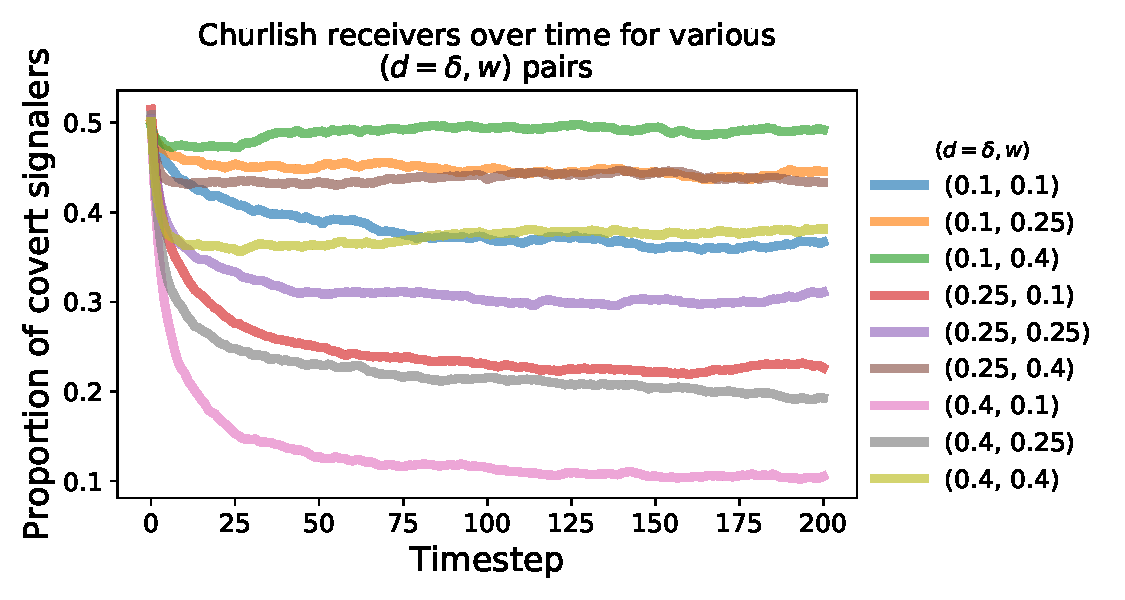
\includegraphics[width=\textwidth]{prelim/Figures/dislikingHomophilyChurlishSeries.pdf}
    \caption{Density of churlish receivers.}
  \end{subfigure}
  
  \caption{Timeseries of density of covert signalers and churlish receivers
    for nine combinations of $d=\delta$ and $w$.}
  \label{fig:dislikingHomophilySeries}
\end{figure}

\begin{figure}[H]
  \centering
  \begin{subfigure}{0.49\textwidth}
    \centering
    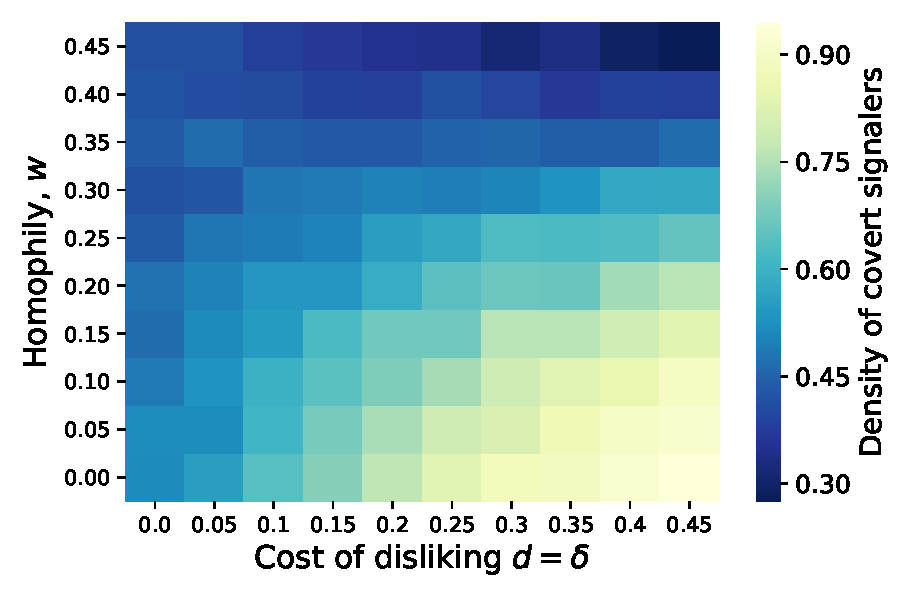
\includegraphics[width=\textwidth]{prelim/Figures/covertDensityVsDislikingHomophilyCoevo.pdf}
    \caption{Density of covert signalers.}
  \end{subfigure}
  \begin{subfigure}{0.49\textwidth}
    \centering
    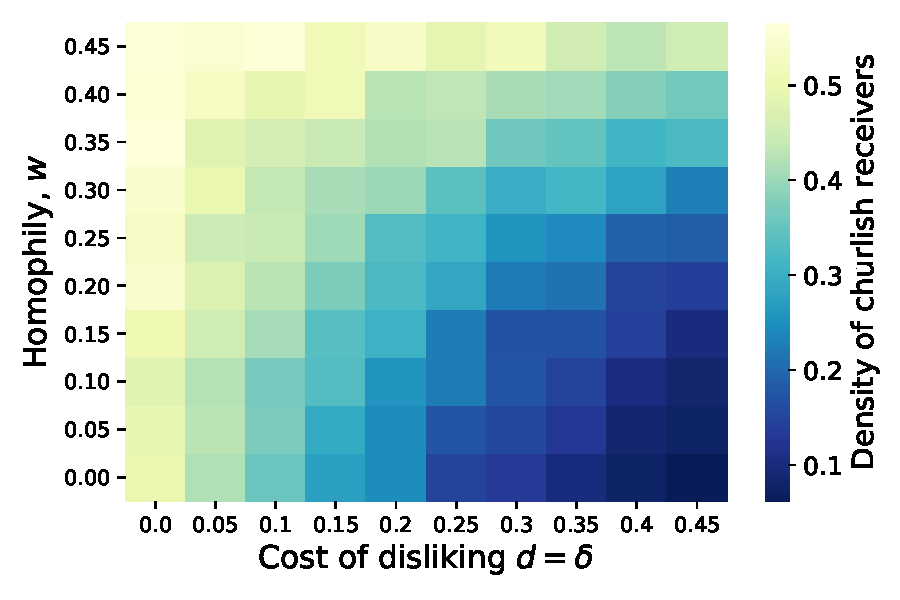
\includegraphics[width=\textwidth]{prelim/Figures/churlishDensityVsDislikingHomophilyCoevo.pdf}
    \caption{Density of churlish receivers.}
  \end{subfigure}
  
  \caption{Density of covert signalers and churlish receivers at $t=200$, 
    final timestep recorded in this preliminary experiment.}
  \label{fig:dislikingHomophilyHeatmap}
\end{figure}


\subsection{Correlations between proportion of covert signalers and of churlish receivers}

\begin{figure}[H]
  \centering
  \begin{subfigure}{0.49\textwidth}
    \centering
    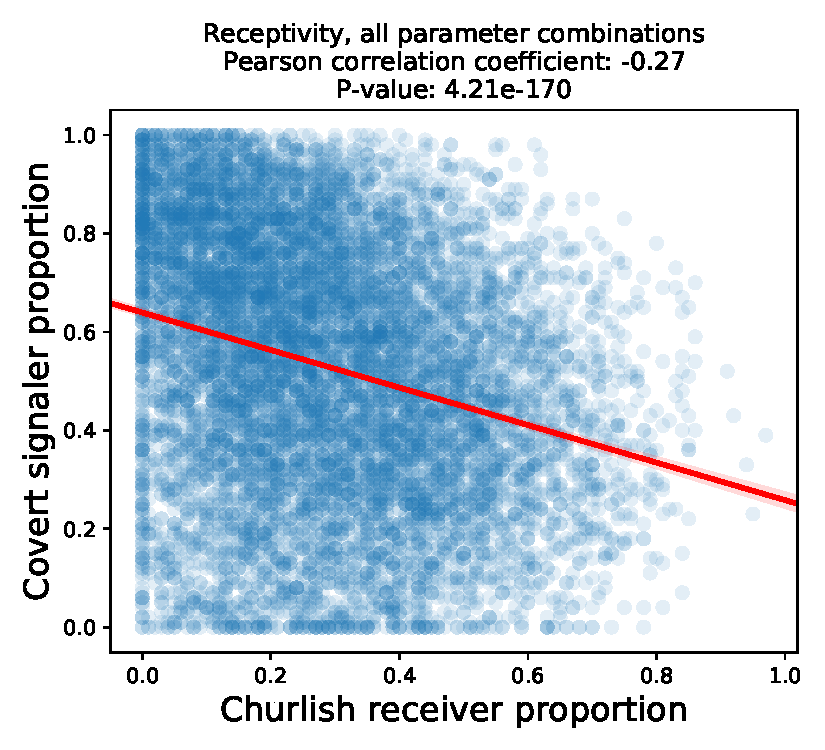
\includegraphics[width=\textwidth]{prelim/Figures/receptivity_allcombos_reg.pdf}
    \caption{}
    \label{fig:}
  \end{subfigure}
  \begin{subfigure}{0.49\textwidth}
    \centering
    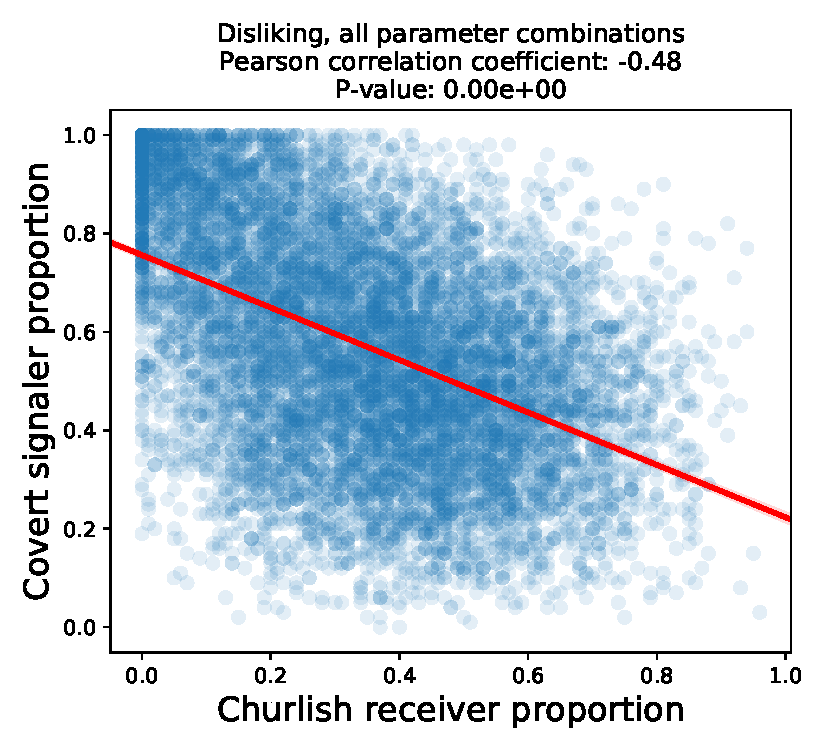
\includegraphics[width=\textwidth]{prelim/Figures/disliking_allcombos_reg.pdf}
    \caption{}
    \label{fig:}
  \end{subfigure}
  \caption{Correlation between proportion of covert signalers and proportion of
    churlish receivers for all tested parameter combinations in both 
    receptivity (a) and disliking (b) experiments.}
  \label{fig:regressions}
\end{figure}


\section{Invasion experiments}

Here we run identical experiments, but vary the initial proportion of 
churlish receivers and covert receivers over $\{0.05, 0.5, 0.95\}$ for a total
of nine parameter combinations. One of these is a repeat of the previous
experiments, where both parameters are set to 0.5. Below are two figures.
The first is nine parameter settings where the density of covert signalers
is plotted in a heatmap (Figure~\ref{fig:invasion-signaling}). The second has 
heatmaps of the density of churlish receivers (Figure~\ref{fig:invasion-receiving}).

\input{prelim/invasion-figures.tex}



\section{Minority populations}

So far in these results I tested the case where a 10\% or 25\% of all agents have
the minority trait, $+1$ in the first trait vector position. 
The other 90\% or 75\% have the majority trait, $-1$ in the first trait vector position.

$r=0.25$, $R=0.5$.

\subsection{Covert signaling}

\subsubsection{Fraction of minorities = 0.10}
\begin{figure}[H]
  \centering
  \begin{subfigure}{0.49\textwidth}
    \centering
    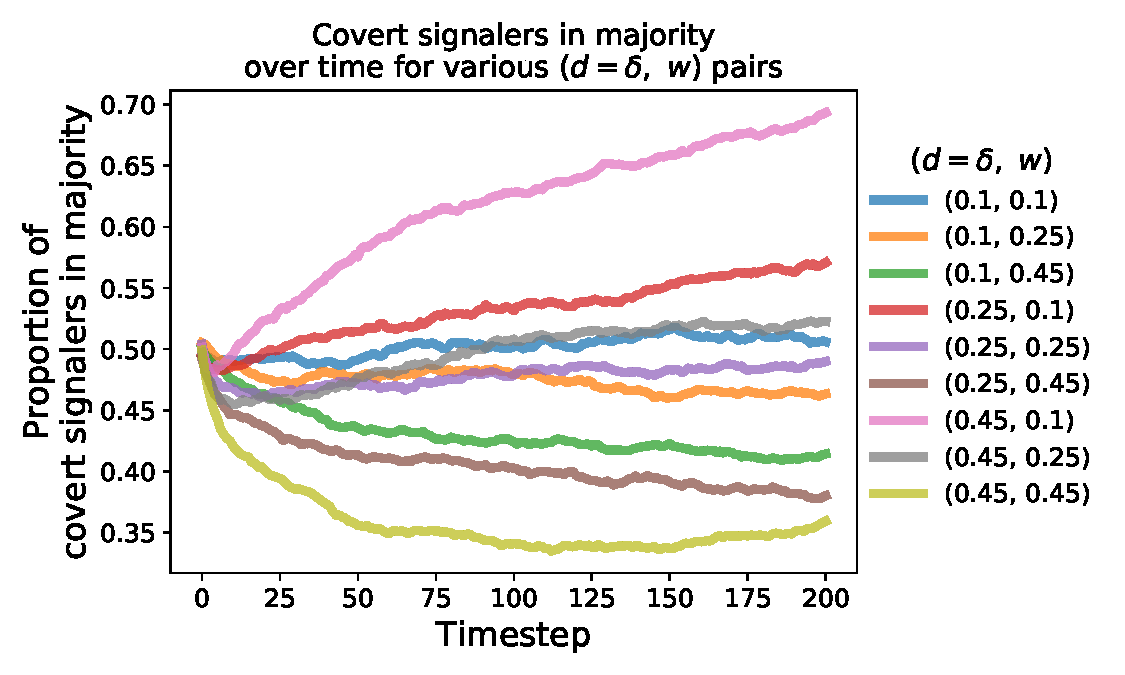
\includegraphics[width=\textwidth]{prelim/Figures/covert_series_majority.pdf}
    \caption{}
    \label{fig:}
  \end{subfigure}
  \begin{subfigure}{0.49\textwidth}
    \centering
    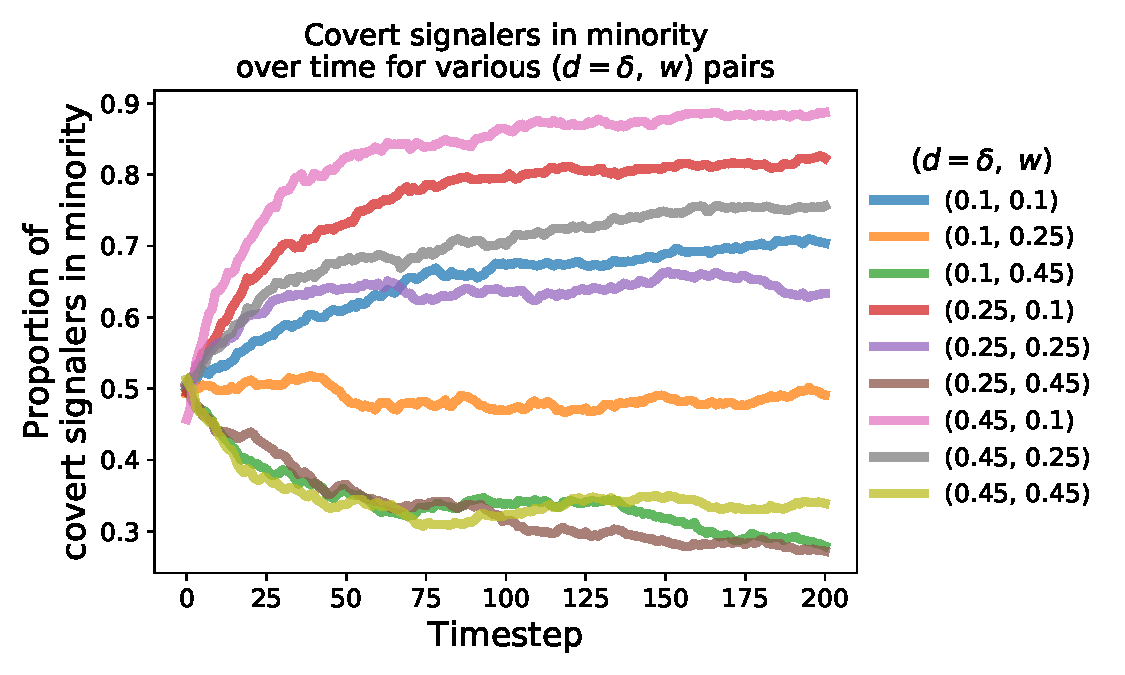
\includegraphics[width=\textwidth]{prelim/Figures/covert_series_minority.pdf}
    \caption{}
    \label{fig:}
  \end{subfigure}
  \caption{Mean timeseries of the evolution of covert signaling in the
    majority (a) and minority (b) populations.}
  \label{fig:}
\end{figure}


\begin{figure}[H]
  \centering
  \begin{subfigure}{0.49\textwidth}
    \centering
    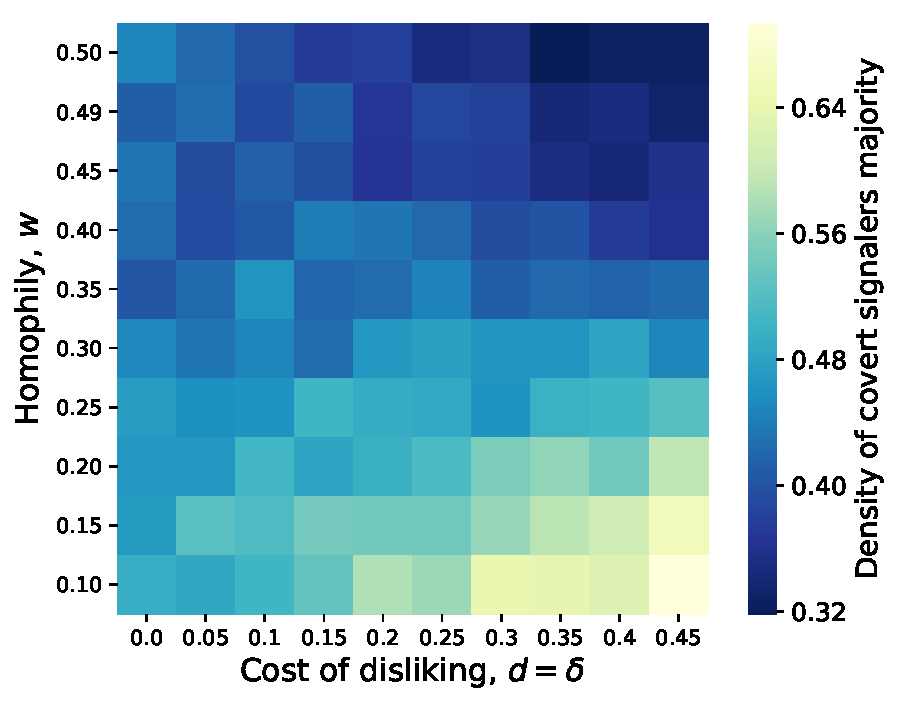
\includegraphics[width=\textwidth]{prelim/Figures/majority_signalers.pdf}
    \caption{}
    \label{fig:}
  \end{subfigure}
  \begin{subfigure}{0.49\textwidth}
    \centering
    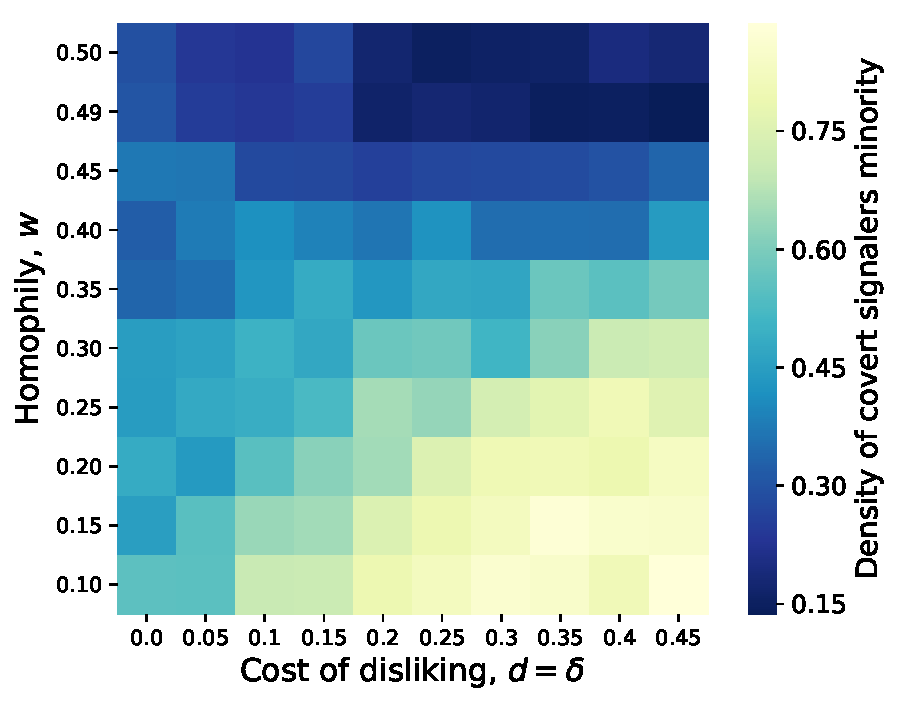
\includegraphics[width=\textwidth]{prelim/Figures/minority_signalers.pdf}
    \caption{}
    \label{fig:}
  \end{subfigure}
  \caption{Proprtion of covert signalers for different parameter settings in the
    majority (a) and minority (b) populations.}
  \label{fig:regressions}
\end{figure}

\begin{figure}[H]
  \centering
    \includegraphics[width=0.6\textwidth]{prelim/Figures/covert_signalers_diff.pdf}
  \caption{Difference between proportion of covert signalers in the minority 
    and majority populations. When cost of disliking is high and homophily is 
    low, more minority agents are covert signalers than majority agents,
    proportionally. An increase in homophily enables minority agents to 
    find one another more easily, so overt signaling, which reaches more of
    the population, is advantageous.
  }
  \label{fig:}
\end{figure}

\subsubsection{Fraction of minorities = 0.25}

\begin{figure}[H]
  \centering
  \begin{subfigure}{0.49\textwidth}
    \centering
    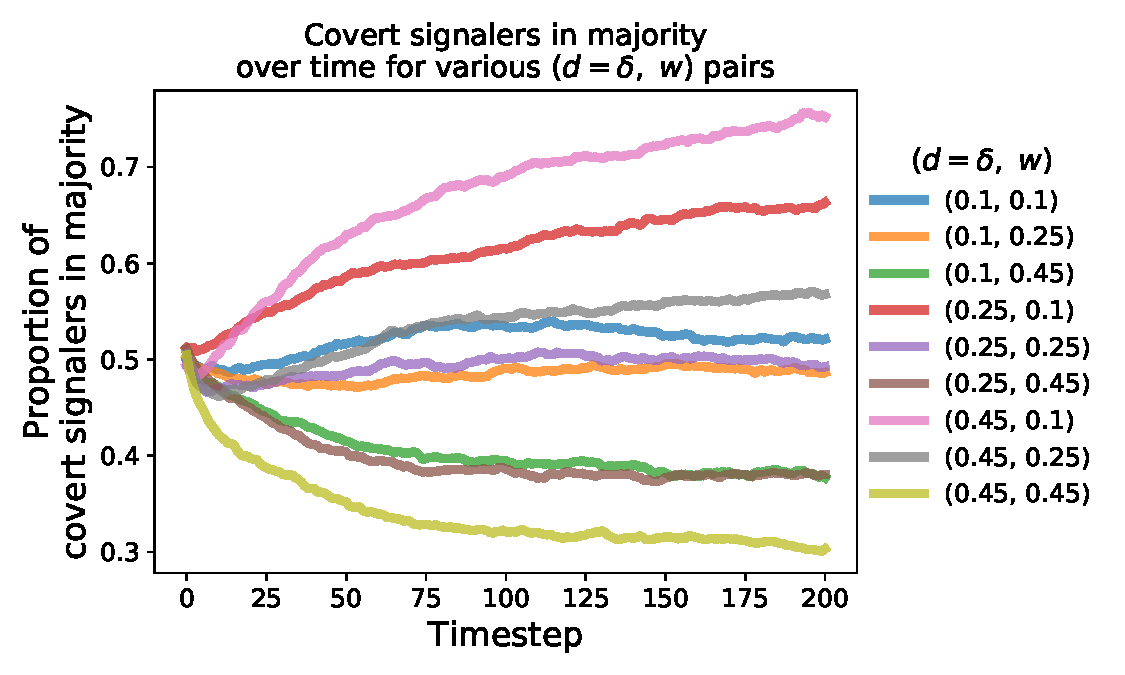
\includegraphics[width=\textwidth]{prelim/Figures/covert_series_majority_025.pdf}
    \caption{}
    \label{fig:}
  \end{subfigure}
  \begin{subfigure}{0.49\textwidth}
    \centering
    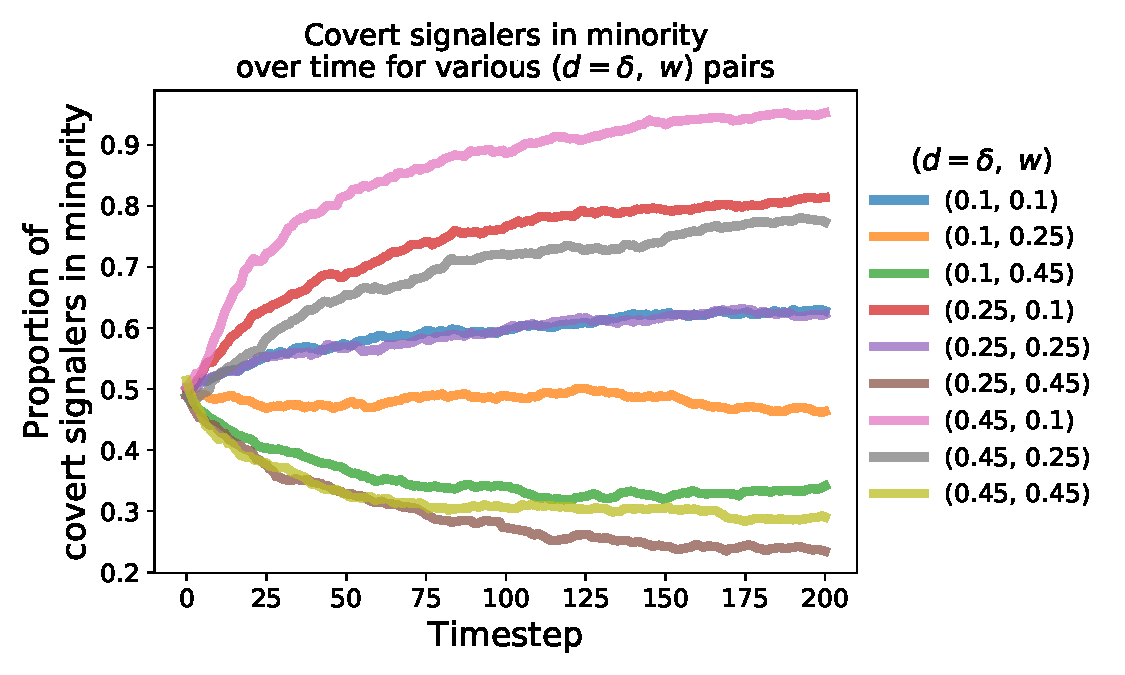
\includegraphics[width=\textwidth]{prelim/Figures/covert_series_minority_025.pdf}
    \caption{}
    \label{fig:}
  \end{subfigure}
  \caption{Mean timeseries of the evolution of covert signaling in the
    majority (a) and minority (b) populations.}
  \label{fig:regressions}
\end{figure}


\begin{figure}[H]
  \centering
  \begin{subfigure}{0.49\textwidth}
    \centering
    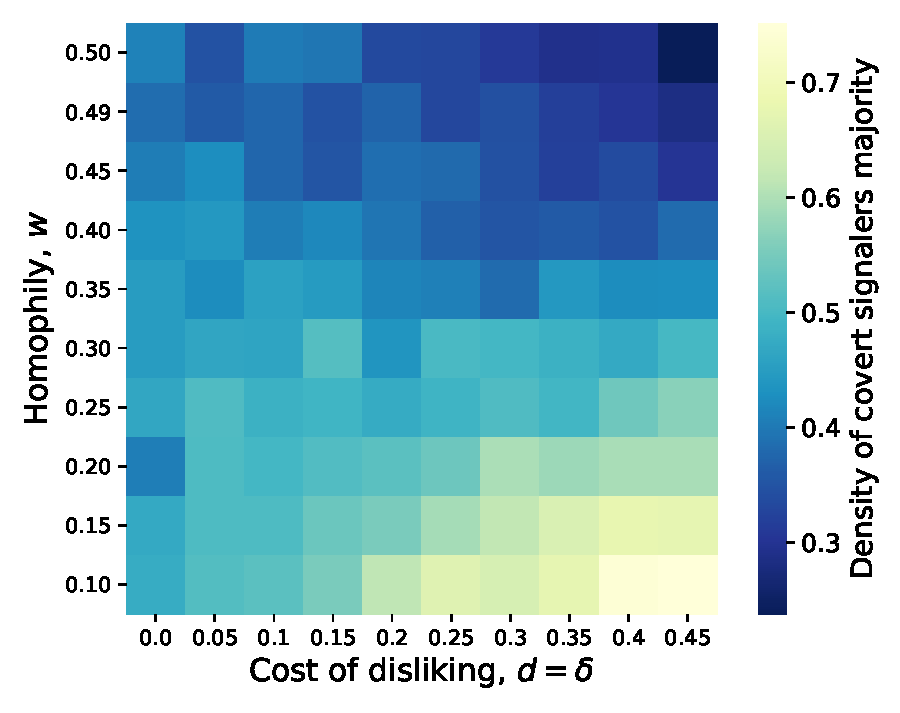
\includegraphics[width=\textwidth]{prelim/Figures/majority_signalers_025.pdf}
    \caption{}
    \label{fig:}
  \end{subfigure}
  \begin{subfigure}{0.49\textwidth}
    \centering
    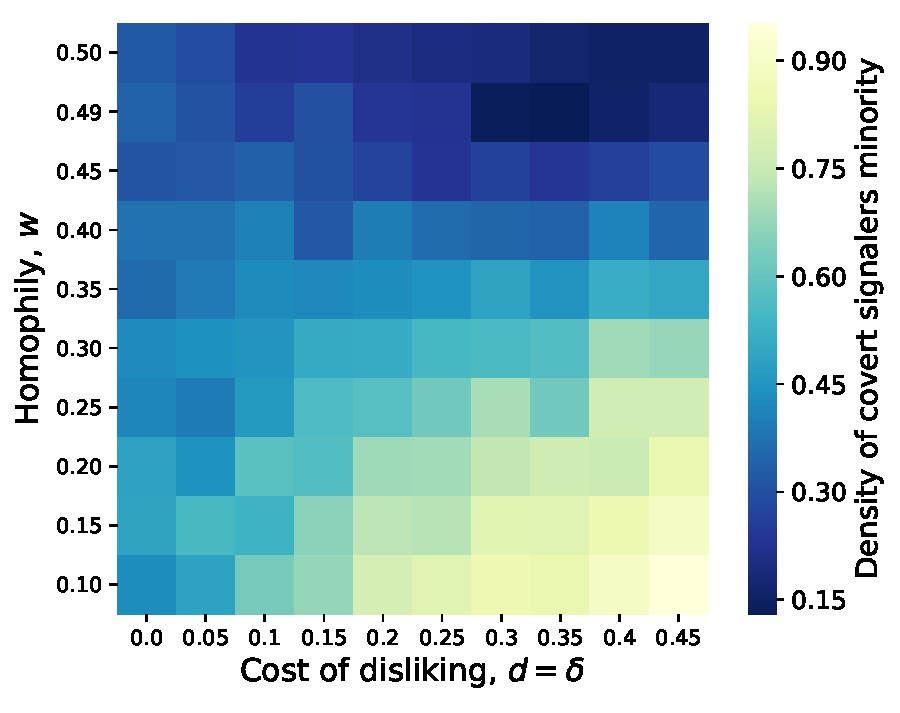
\includegraphics[width=\textwidth]{prelim/Figures/minority_signalers_025.pdf}
    \caption{}
    \label{fig:}
  \end{subfigure}
  \caption{Proprtion of covert signalers for different parameter settings in the
    majority (a) and minority (b) populations.}
  \label{fig:regressions}
\end{figure}

\begin{figure}[H]
  \centering
    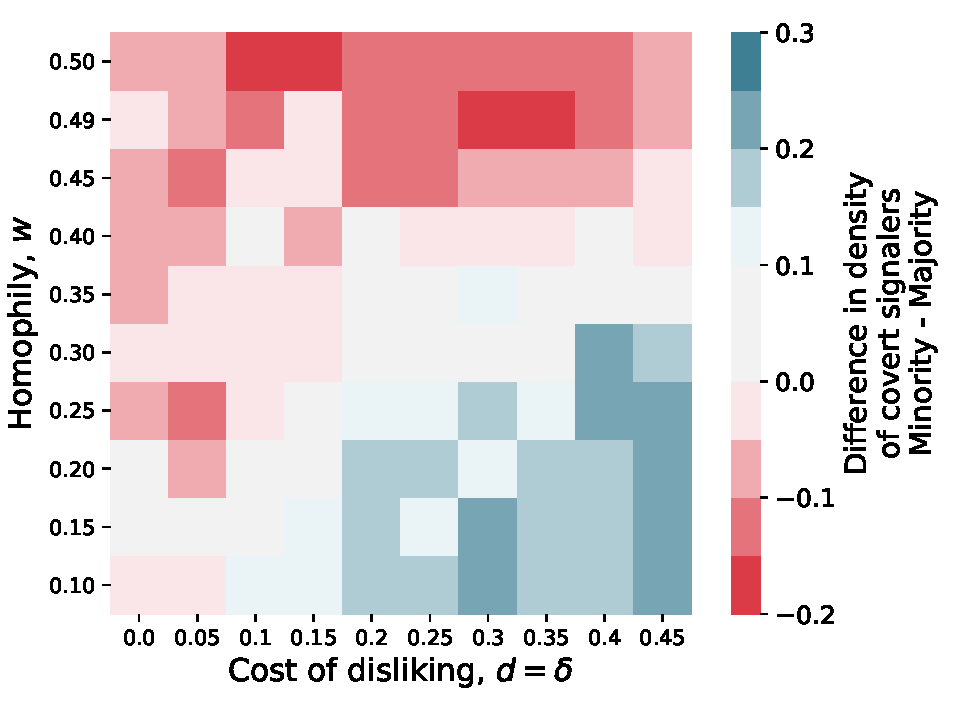
\includegraphics[width=0.6\textwidth]{prelim/Figures/covert_signalers_diff_025.pdf}
  \caption{Difference between proportion of covert signalers in the minority 
    and majority populations. When cost of disliking is high and homophily is 
    low, more minority agents are covert signalers than majority agents,
    proportionally. An increase in homophily enables minority agents to 
    find one another more easily, so overt signaling, which reaches more of
    the population, is advantageous.
  }
  \label{fig:}
\end{figure}

\subsubsection{Fraction of minorities = 0.05}

\begin{figure}[H]
  \centering
  \begin{subfigure}{0.49\textwidth}
    \centering
    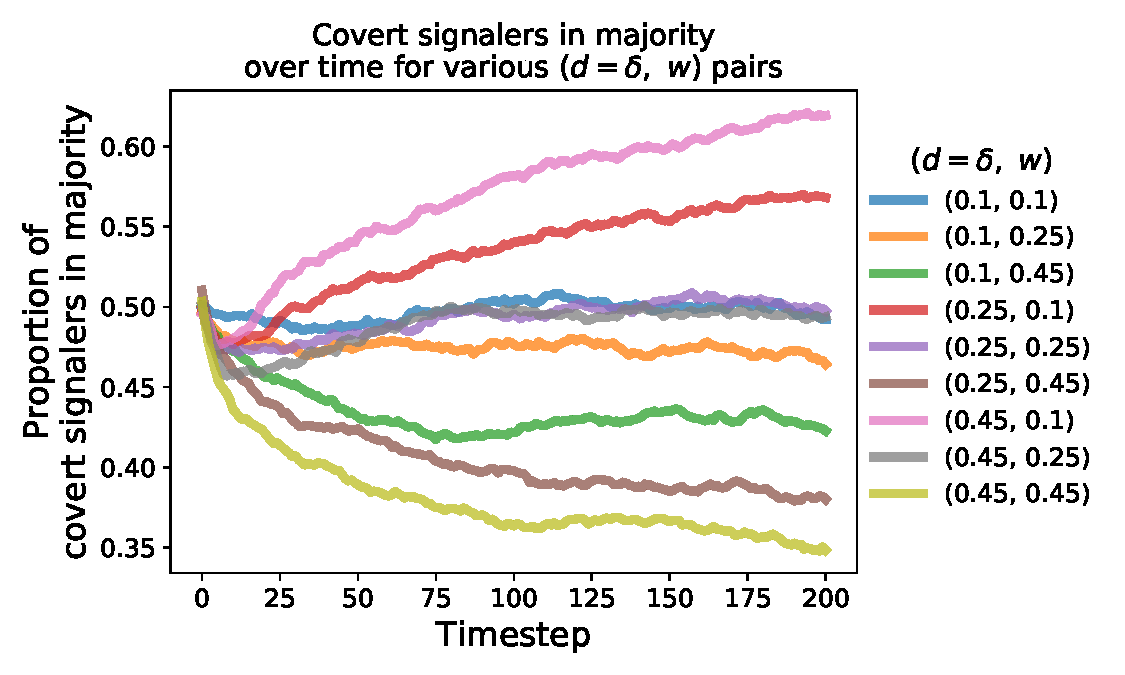
\includegraphics[width=\textwidth]{prelim/Figures/covert_series_majority_005.pdf}
    \caption{}
    \label{fig:}
  \end{subfigure}
  \begin{subfigure}{0.49\textwidth}
    \centering
    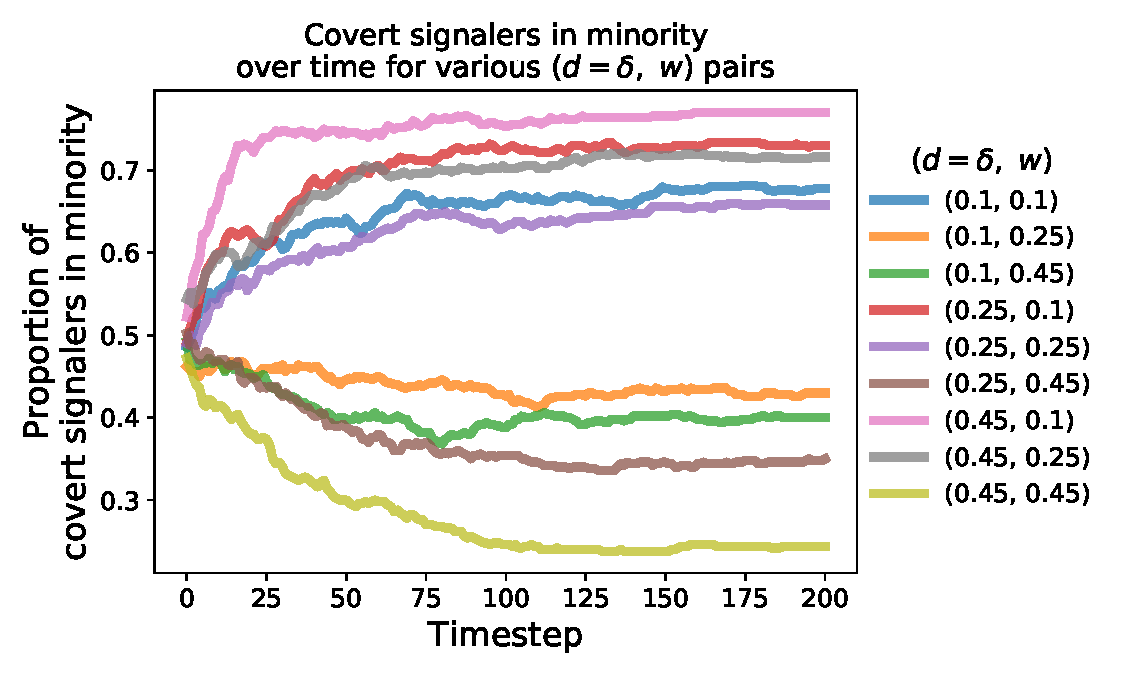
\includegraphics[width=\textwidth]{prelim/Figures/covert_series_minority_005.pdf}
    \caption{}
    \label{fig:}
  \end{subfigure}
  \caption{Mean timeseries of the evolution of covert signaling in the
    majority (a) and minority (b) populations.}
  \label{fig:regressions}
\end{figure}


\begin{figure}[H]
  \centering
  \begin{subfigure}{0.49\textwidth}
    \centering
    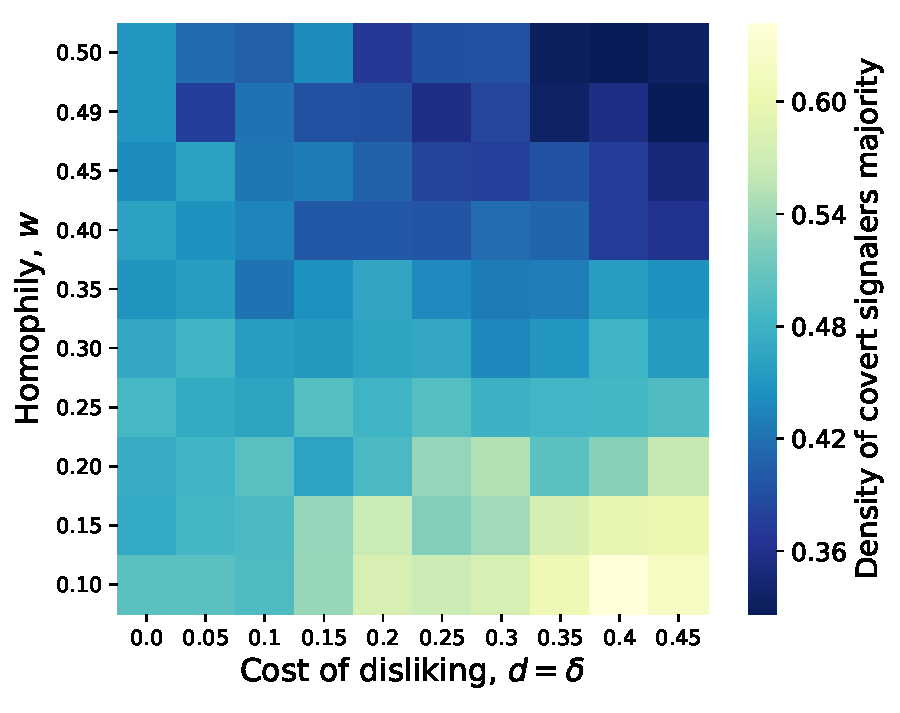
\includegraphics[width=\textwidth]{prelim/Figures/majority_signalers_005.pdf}
    \caption{}
    \label{fig:}
  \end{subfigure}
  \begin{subfigure}{0.49\textwidth}
    \centering
    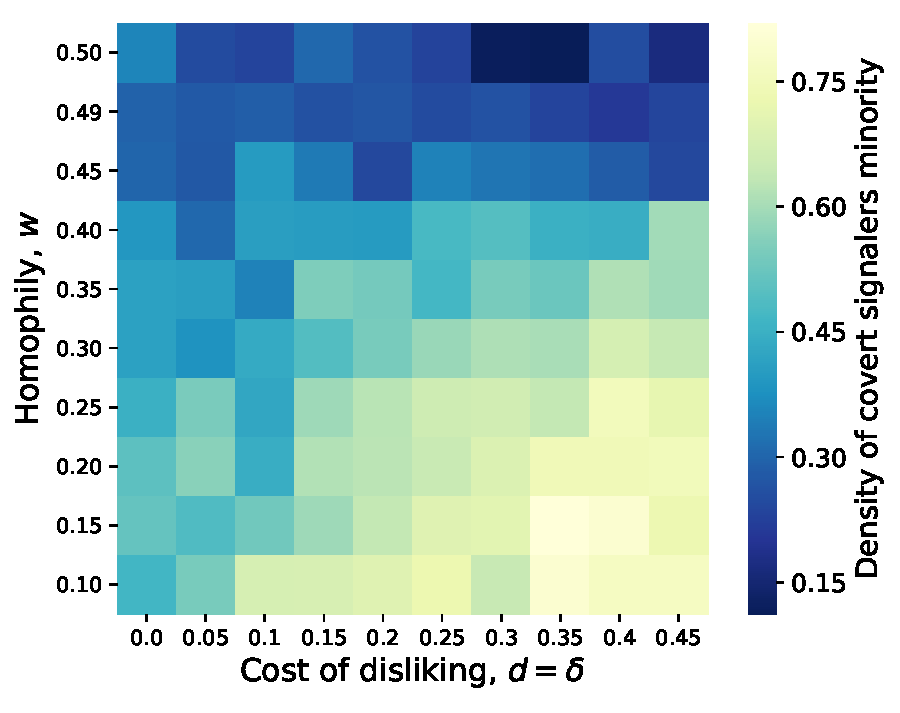
\includegraphics[width=\textwidth]{prelim/Figures/minority_signalers_005.pdf}
    \caption{}
    \label{fig:}
  \end{subfigure}
  \caption{Proprtion of covert signalers for different parameter settings in the
    majority (a) and minority (b) populations.}
  \label{fig:regressions}
\end{figure}

\begin{figure}[H]
  \centering
    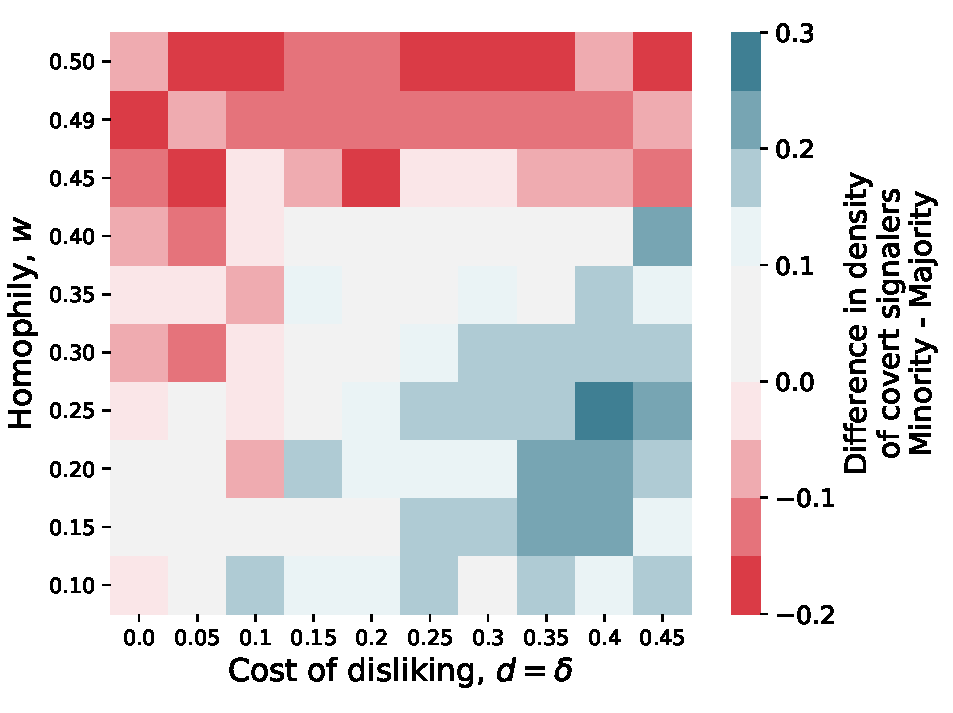
\includegraphics[width=0.6\textwidth]{prelim/Figures/covert_signalers_diff_005.pdf}
  \caption{Difference between proportion of covert signalers in the minority 
    and majority populations. When cost of disliking is high and homophily is 
    low, more minority agents are covert signalers than majority agents,
    proportionally. An increase in homophily enables minority agents to 
    find one another more easily, so overt signaling, which reaches more of
    the population, is advantageous.
  }
  \label{fig:}
\end{figure}


\subsection{Churlish receiving}

\subsubsection{Fraction of minorities = 0.10}

\begin{figure}[H]
  \centering
  \begin{subfigure}{0.49\textwidth}
    \centering
    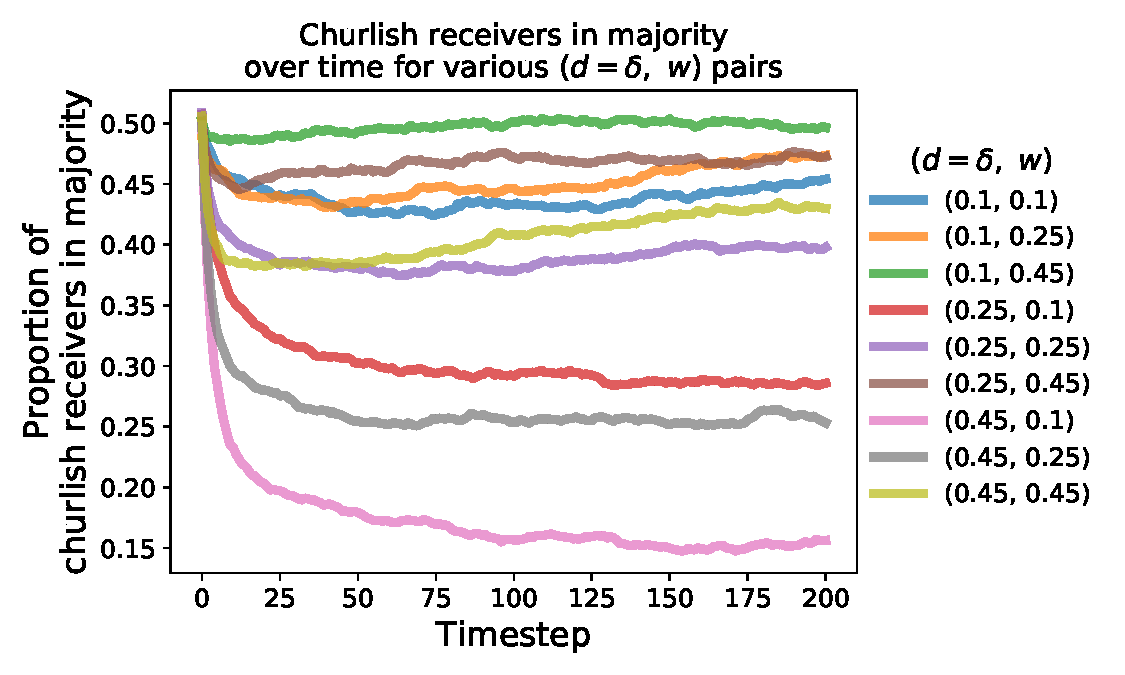
\includegraphics[width=\textwidth]{prelim/Figures/churlish_series_majority.pdf}
    \caption{}
    \label{fig:}
  \end{subfigure}
  \begin{subfigure}{0.49\textwidth}
    \centering
    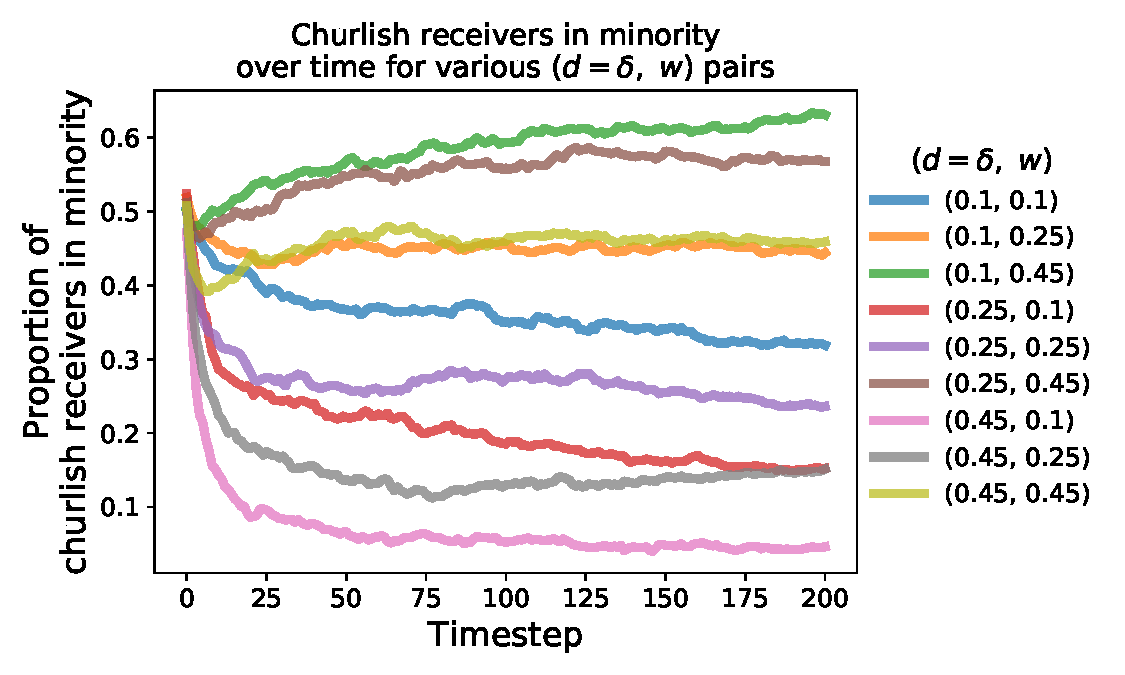
\includegraphics[width=\textwidth]{prelim/Figures/churlish_series_minority.pdf}
    \caption{}
    \label{fig:}
  \end{subfigure}
  \caption{Mean timeseries of the evolution of churlish receiving in the
    majority (a) and minority (b) populations.}
  \label{fig:regressions}
\end{figure}


\begin{figure}[H]
  \centering
  \begin{subfigure}{0.49\textwidth}
    \centering
    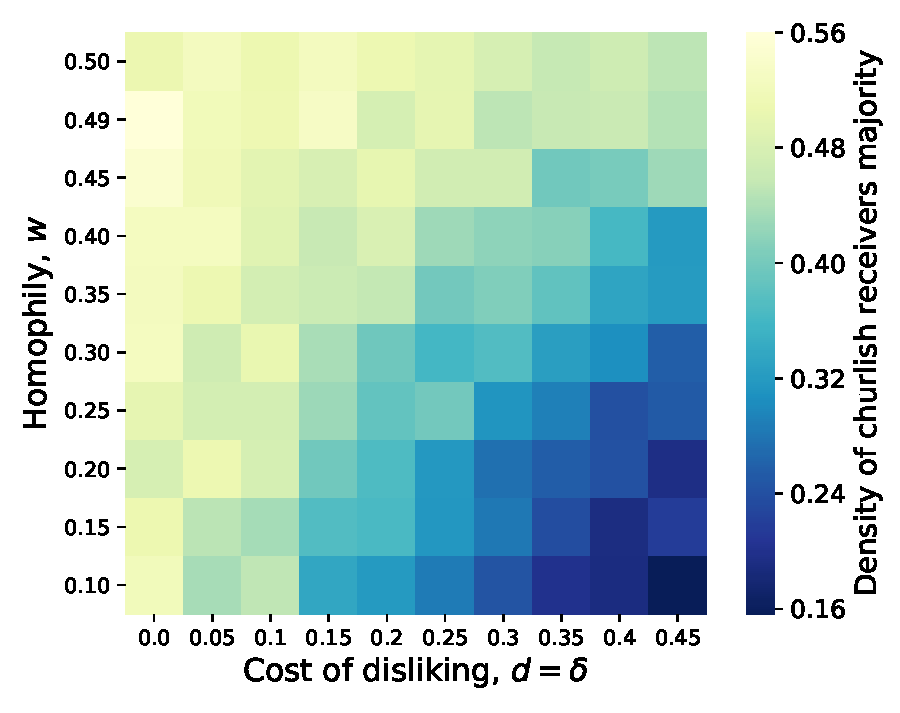
\includegraphics[width=\textwidth]{prelim/Figures/majority_receivers.pdf}
    \caption{}
    \label{fig:}
  \end{subfigure}
  \begin{subfigure}{0.49\textwidth}
    \centering
    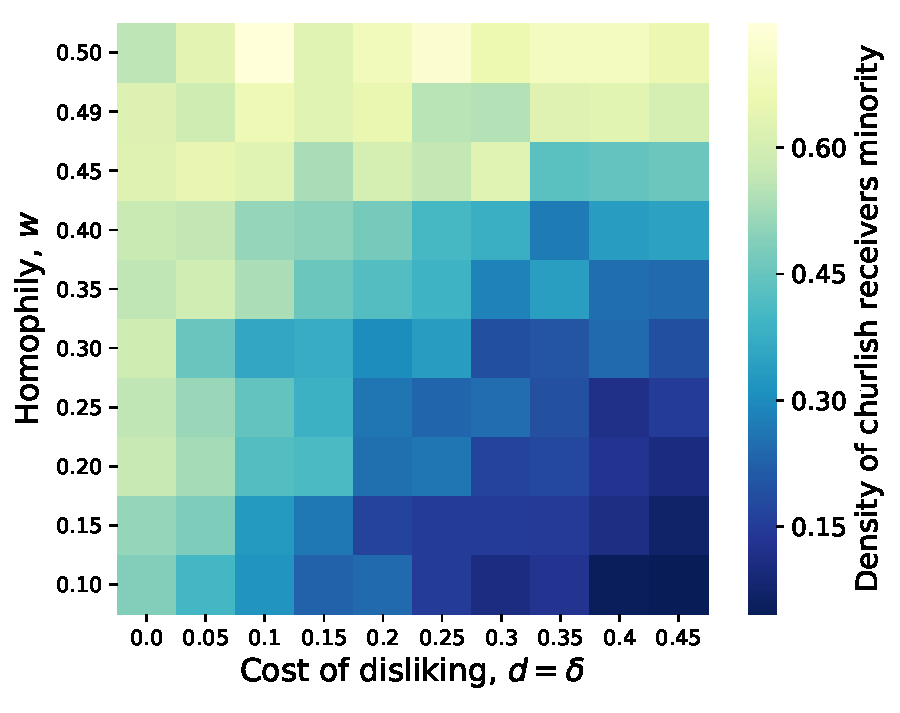
\includegraphics[width=\textwidth]{prelim/Figures/minority_receivers.pdf}
    \caption{}
    \label{fig:}
  \end{subfigure}
  \caption{Proprtion of churlish receivers for different parameter settings in the
    majority (a) and minority (b) populations.}
  \label{fig:regressions}
\end{figure}

\begin{figure}[H]
  \centering
    \includegraphics[width=0.6\textwidth]{prelim/Figures/churlish_receivers_diff.pdf}
  \caption{Difference between proportion of churlish receivers in the minority 
    and majority populations. Here the dependence is primarily on homophily.
    If homophily is too low, the minority population cannot interact often
    enough with their in-group, and so must adopt a non-churlish stance towards
    others in order to not suffer cost of disliking penalties. Once the minority
    can reliably find its in-group members (increasing homophily) the minority
    can afford to assume they dislike others, since by and large they dislike
    the majority.
  }
  \label{fig:}
\end{figure}


\subsubsection{Fraction of minorities = 0.25}

\begin{figure}[H]
  \centering
  \begin{subfigure}{0.49\textwidth}
    \centering
    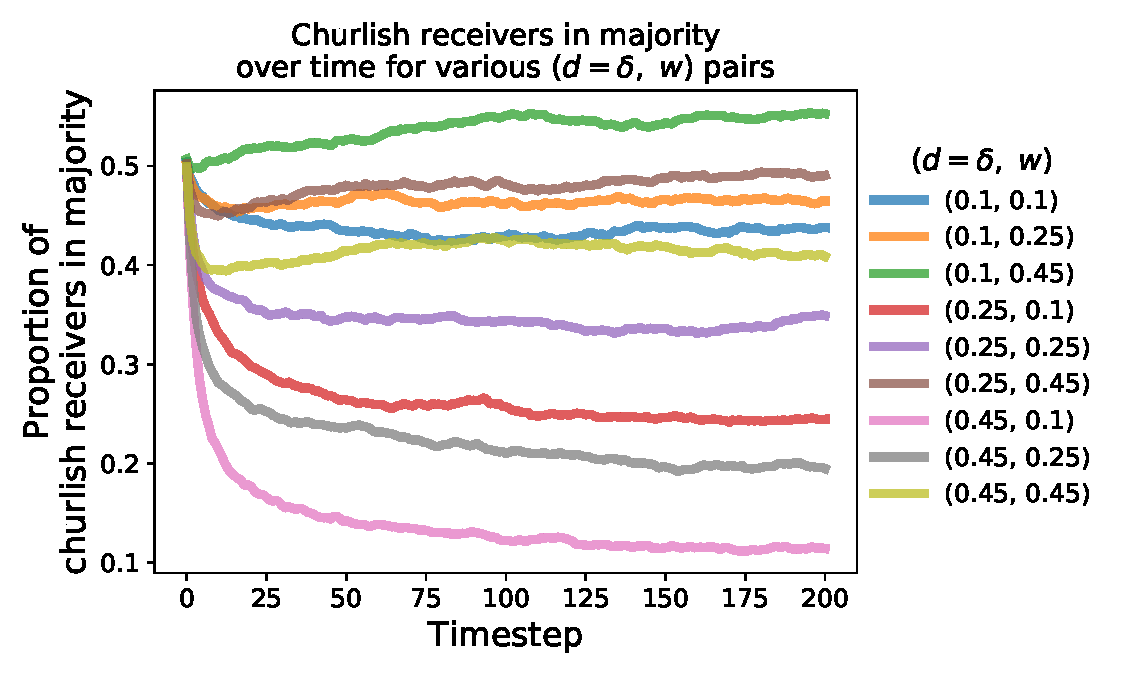
\includegraphics[width=\textwidth]{prelim/Figures/churlish_series_majority_025.pdf}
    \caption{}
    \label{fig:}
  \end{subfigure}
  \begin{subfigure}{0.49\textwidth}
    \centering
    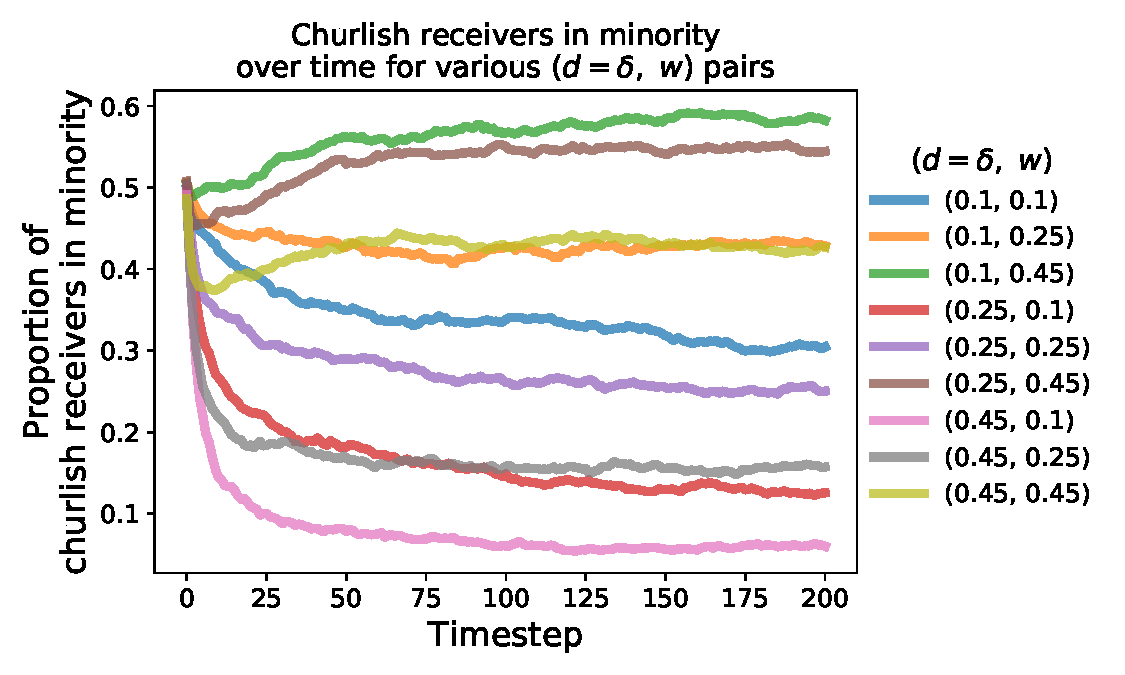
\includegraphics[width=\textwidth]{prelim/Figures/churlish_series_minority_025.pdf}
    \caption{}
    \label{fig:}
  \end{subfigure}
  \caption{Mean timeseries of the evolution of churlish receiving in the
    majority (a) and minority (b) populations.}
  \label{fig:regressions}
\end{figure}


\begin{figure}[H]
  \centering
  \begin{subfigure}{0.49\textwidth}
    \centering
    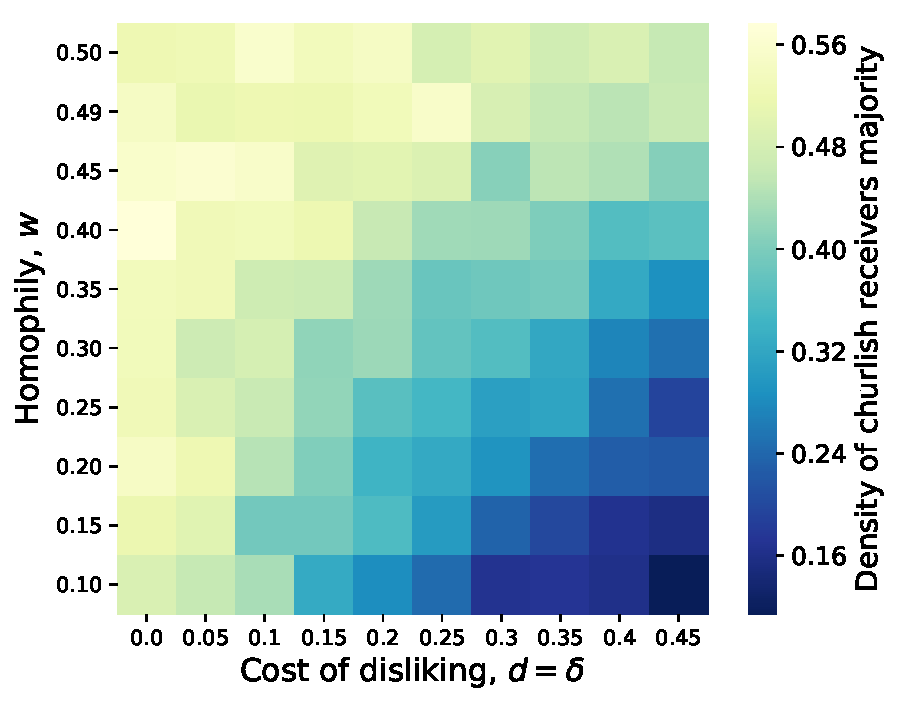
\includegraphics[width=\textwidth]{prelim/Figures/majority_receivers_025.pdf}
    \caption{}
    \label{fig:}
  \end{subfigure}
  \begin{subfigure}{0.49\textwidth}
    \centering
    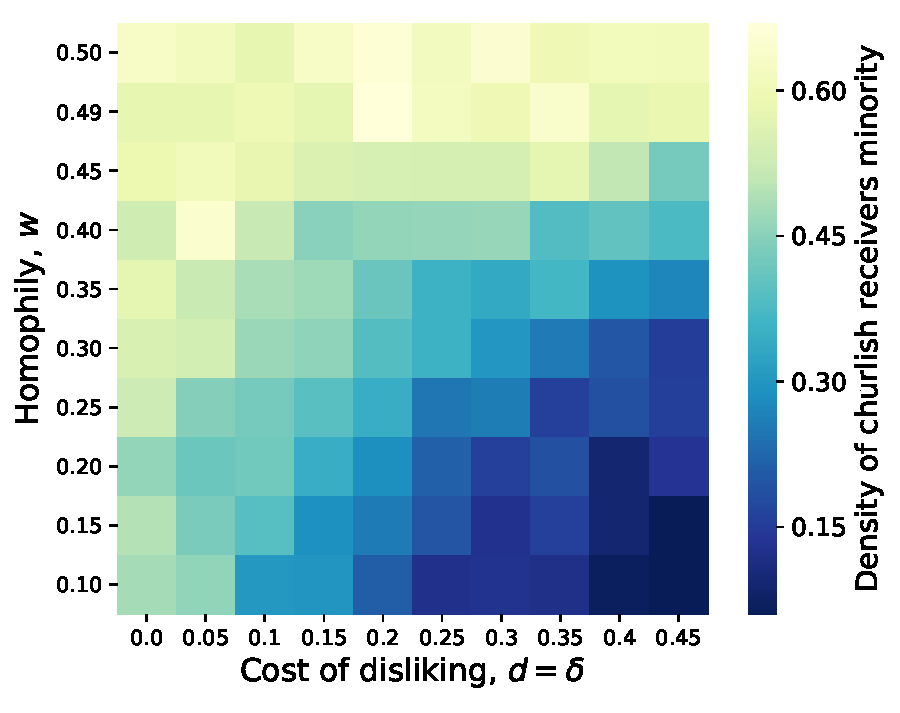
\includegraphics[width=\textwidth]{prelim/Figures/minority_receivers_025.pdf}
    \caption{}
    \label{fig:}
  \end{subfigure}
  \caption{Proprtion of churlish receivers for different parameter settings in the
    majority (a) and minority (b) populations.}
  \label{fig:regressions}
\end{figure}

\begin{figure}[H]
  \centering
    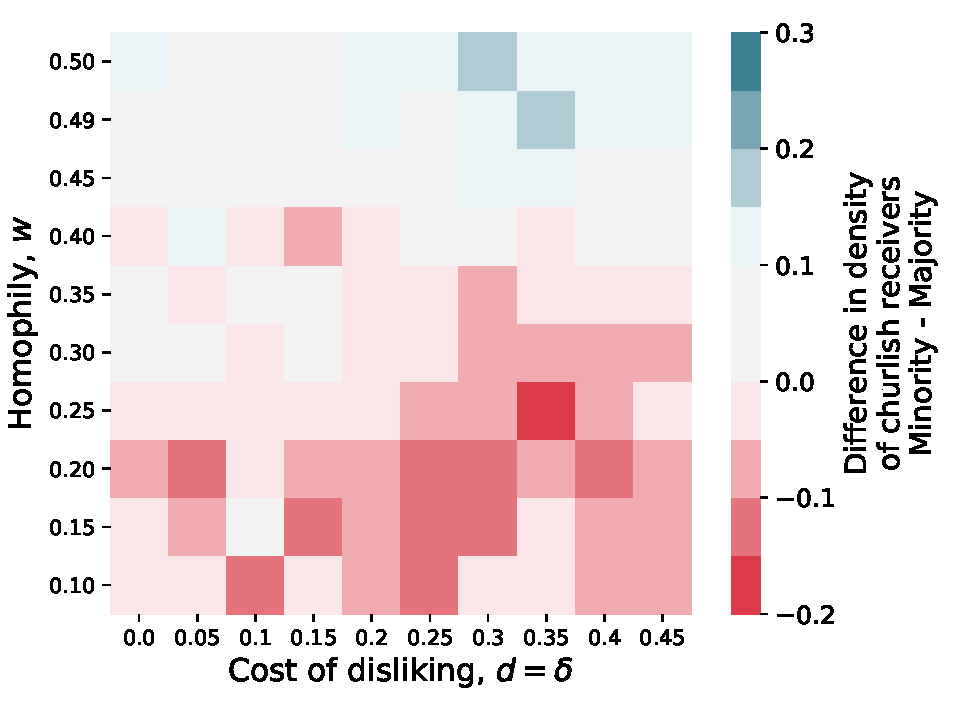
\includegraphics[width=0.6\textwidth]{prelim/Figures/churlish_receivers_diff_025.pdf}
  \caption{Difference between proportion of churlish receivers in the minority 
    and majority populations. Here the dependence is primarily on homophily.
    If homophily is too low, the minority population cannot interact often
    enough with their in-group, and so must adopt a non-churlish stance towards
    others in order to not suffer cost of disliking penalties. Once the minority
    can reliably find its in-group members (increasing homophily) the minority
    can afford to assume they dislike others, since by and large they dislike
    the majority.
  }
  \label{fig:}
\end{figure}


\subsubsection{Fraction of minorities = 0.05}

\begin{figure}[H]
  \centering
  \begin{subfigure}{0.49\textwidth}
    \centering
    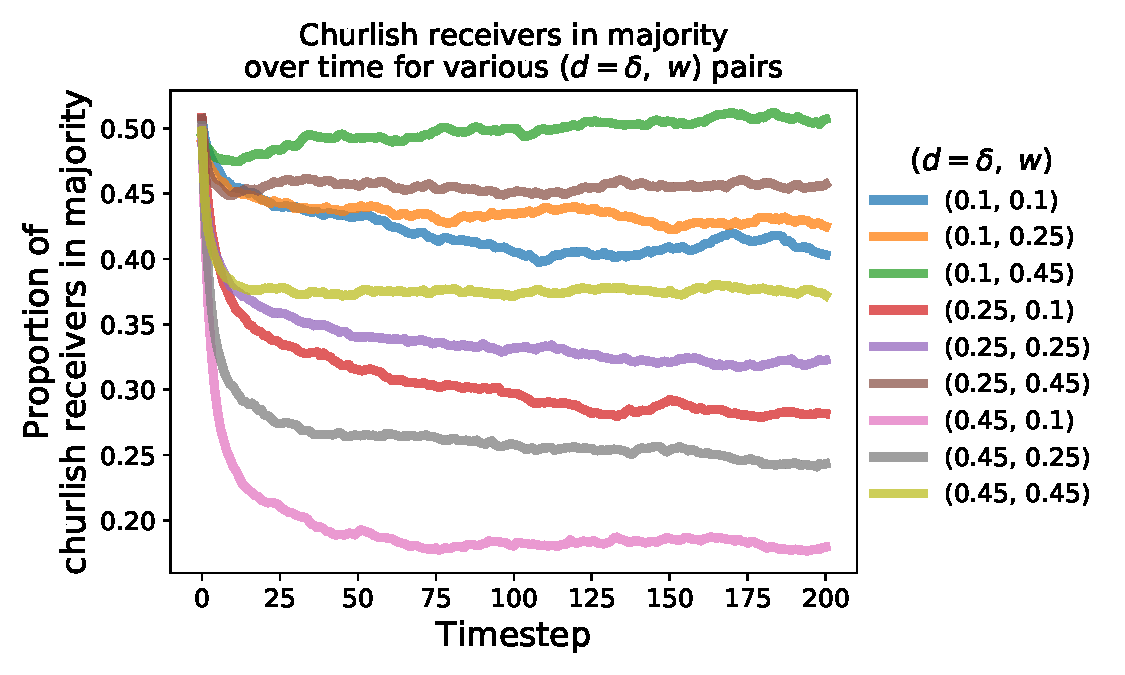
\includegraphics[width=\textwidth]{prelim/Figures/churlish_series_majority_005.pdf}
    \caption{}
    \label{fig:}
  \end{subfigure}
  \begin{subfigure}{0.49\textwidth}
    \centering
    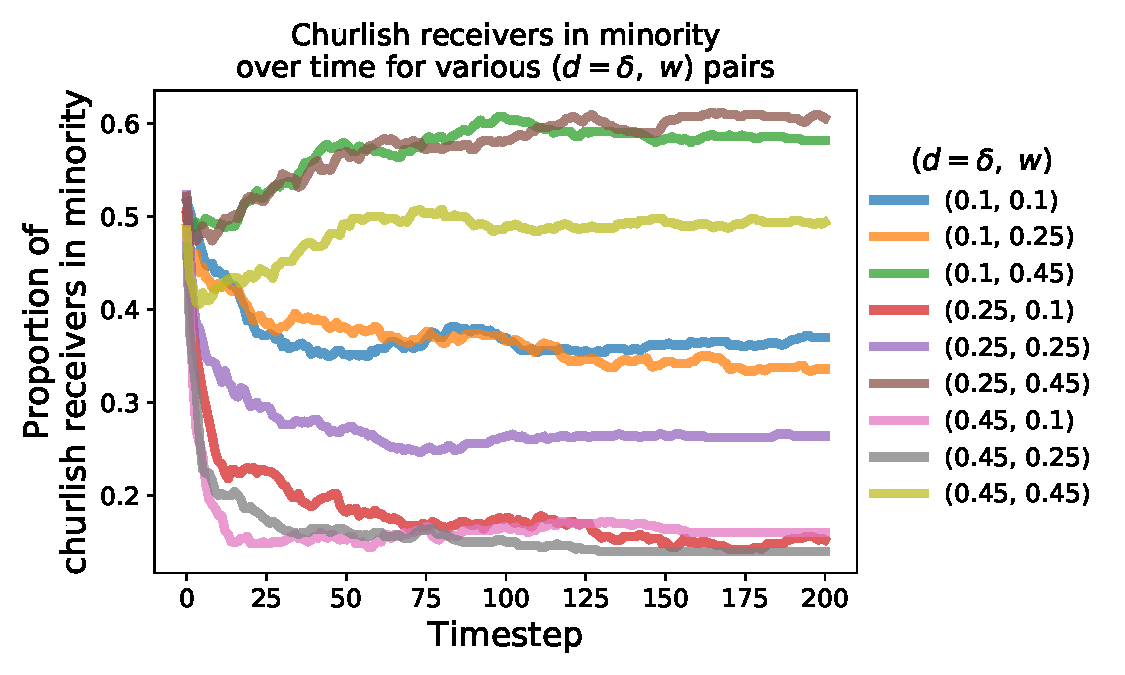
\includegraphics[width=\textwidth]{prelim/Figures/churlish_series_minority_005.pdf}
    \caption{}
    \label{fig:}
  \end{subfigure}
  \caption{Mean timeseries of the evolution of churlish receiving in the
    majority (a) and minority (b) populations.}
  \label{fig:regressions}
\end{figure}


\begin{figure}[H]
  \centering
  \begin{subfigure}{0.49\textwidth}
    \centering
    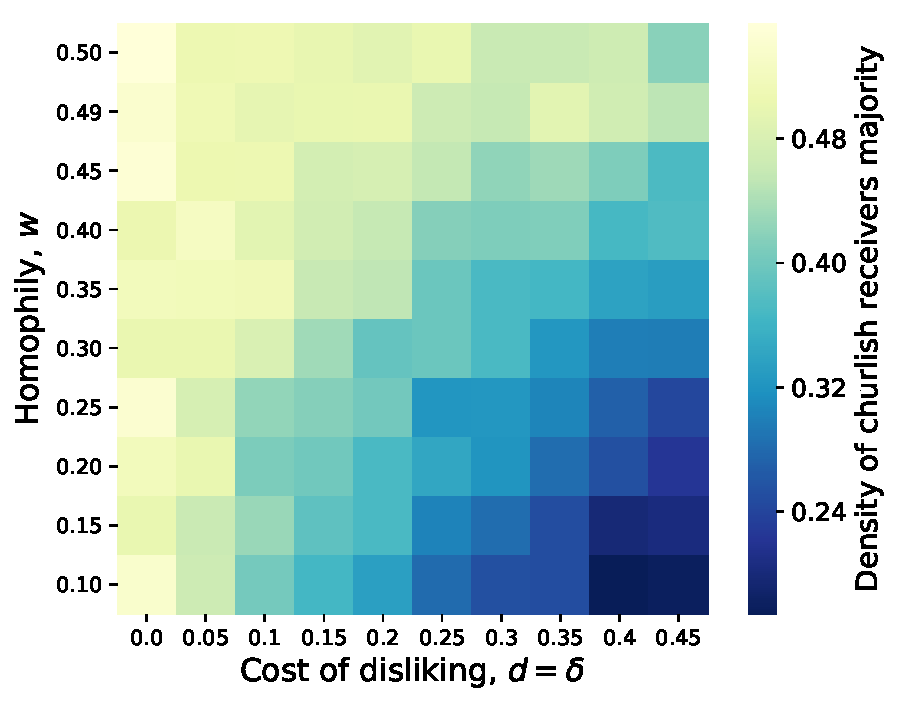
\includegraphics[width=\textwidth]{prelim/Figures/majority_receivers_005.pdf}
    \caption{}
    \label{fig:}
  \end{subfigure}
  \begin{subfigure}{0.49\textwidth}
    \centering
    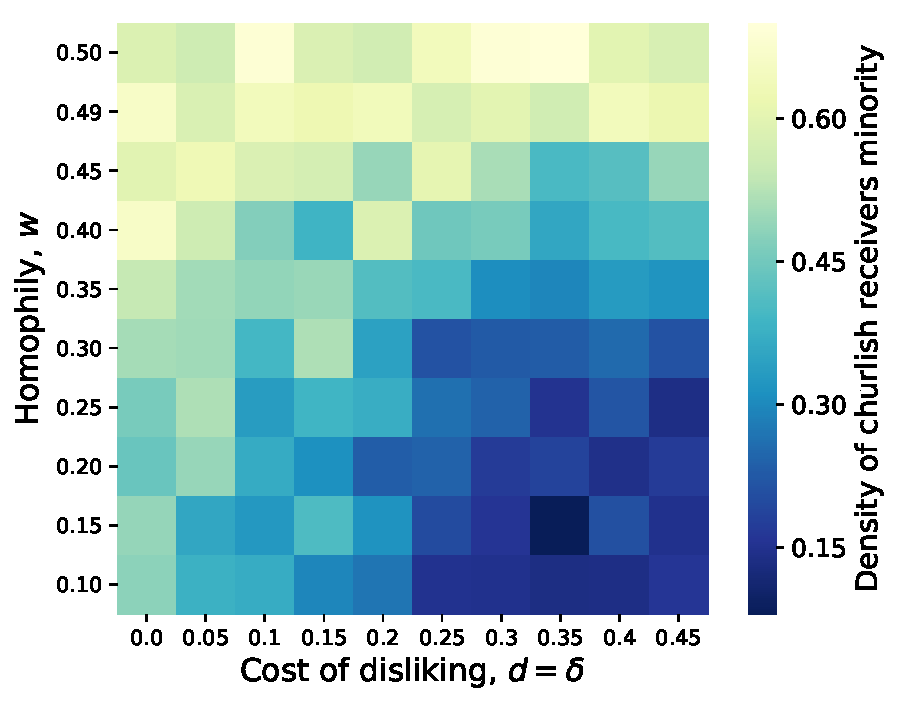
\includegraphics[width=\textwidth]{prelim/Figures/minority_receivers_005.pdf}
    \caption{}
    \label{fig:}
  \end{subfigure}
  \caption{Proprtion of churlish receivers for different parameter settings in the
    majority (a) and minority (b) populations.}
  \label{fig:regressions}
\end{figure}

\begin{figure}[H]
  \centering
    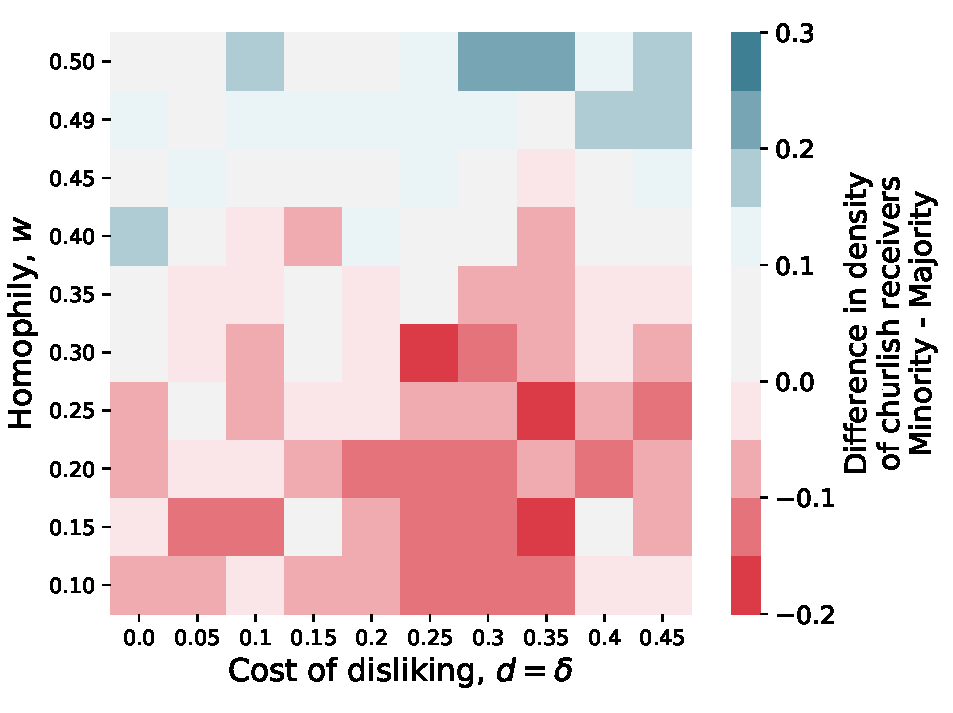
\includegraphics[width=0.6\textwidth]{prelim/Figures/churlish_receivers_diff_005.pdf}
  \caption{Difference between proportion of churlish receivers in the minority 
    and majority populations. Here the dependence is primarily on homophily.
    If homophily is too low, the minority population cannot interact often
    enough with their in-group, and so must adopt a non-churlish stance towards
    others in order to not suffer cost of disliking penalties. Once the minority
    can reliably find its in-group members (increasing homophily) the minority
    can afford to assume they dislike others, since by and large they dislike
    the majority.
  }
  \label{fig:}
\end{figure}


% \section{Discussion}

% These preliminary experiments and results are based on one major finding from
% ECS that covert signaling is maintained when overt signalers do not have
% too large an advantage in the free choice context. ``This requires that
% assortment with liked individuals not be too accurate,'' which corresponds to
% small $w$ in this ABM version. ``The accuracy of assortment is influenced
% by the reception probabilities of both signal types, $R$ and $r$'' (see p.
% 4 in ECS). Our preliminary results find the same trend with our ABM.


% \bibliographystyle{apacite}

% \setlength{\bibleftmargin}{.125in}
% \setlength{\bibindent}{-\bibleftmargin}

% \bibliography{/Users/mt/workspace/papers/library.bib}

\end{document}
